\section{Global Fit Studies}
\label{sec:globalFitStudies}
\subsection{Bin Rescaling}
\label{subsec:binRescaling:GlobalFitting}
The dijet fit functions used are based upon motivation from parton distribution functions $\left(1-\frac{m_{jj}}{\sqrt{S}}\right)^{P_{1}}$ and LO matrix element from QCD dijet MC $\frac{m_{jj}}{\sqrt{S}}^{P_{2}}$ with additional ad-hoc terms determined empirically to account for higher orders %\cite{ATL-COM-PHYS-2018-161}, and ensuring that the function is smooth and monotonically decreasing. 

If the underlying data follows this distribution, variable binning will introduce an artificial deviation in the measured data away from this distribution. Shown in Figure \ref{fig:BinningShapeAdjustment} using events selected from the string resonance cuts, is a ratio between the measured data in events per bin basis and the measured data in events / GeV per bin by dividing by bin width, normalized to be equal in the 7904-8055 GeV bin for comparison. It can be seen that the variable binning introduces a change in shape as expected particularly affecting the low $m_{jj}$ region, and as well as this there are noticeable unsmooth jumps in the distribution coming from the raw events per bin case due to requirements of integer bin widths. Due to this change in shape and unsmooth jumps, to reliably fit the dijet fit functions to data it is required to correct for this, either by using non-variable binning for fits or by a bin rescaling procedure:

\begin{itemize}
    \item Rescale number of events per bin from events to events / GeV via dividing each bin by bin width.
    \item Fit the events / GeV distribution.
    \item Take the value of the fit at the centre of each bin.
    \item Scale this value back to events per bin via multiplying each value by bin width.
\end{itemize}

Shown in Figure \ref{fig:5ParamGlobalFitBinRescaleComparison} is a comparison for the 5 parameter dijet function globally fitted using MINUIT2 to the measured events per bin, and with performing the bin rescaling procedure. The measured $\frac{\chi^{2}}{nDoF}$ of the fit is improved via this bin rescaling procedure by a factor of 20 from 1617/80 to 63.4/80, and in addition it can be seen by eye that without performing this procedure the fit underestimates almost all bins above 5 TeV, while this does not occur when the bin rescaling procedure is applied. Comparisons for additional fit functions and different fitting ranges are available in {\href{https://indico.cern.ch/event/997813/contributions/4191921/attachments/2178521/3679266/dijet_CompareBinRescale_26_01_2021.pdf}{https://indico.cern.ch/event/997813/contributions/4191921/}}.


%\begin{figure}
%    \centering
%    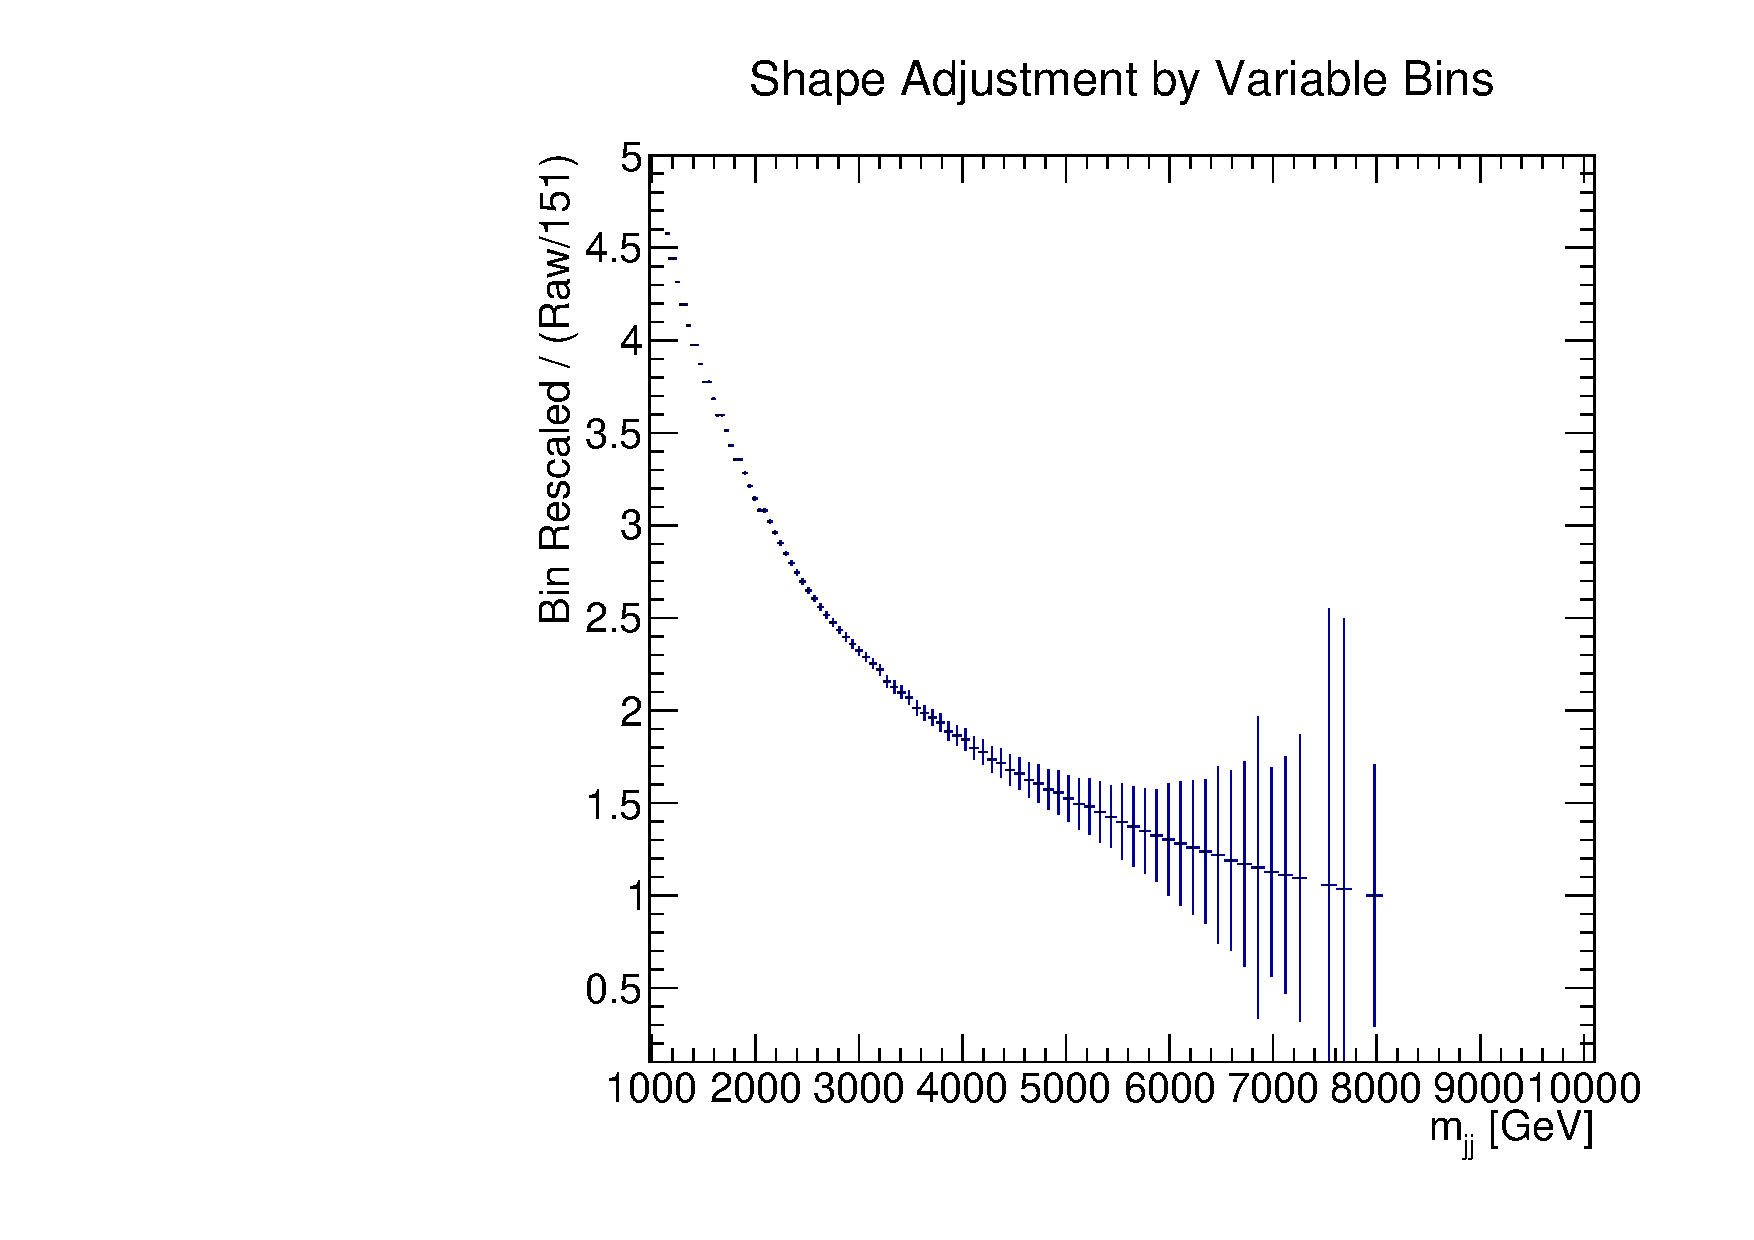
\includegraphics[trim=3 8 35 48, clip,width=1.0\linewidth]{figures/app-GlobalFitStudies/BinningShapeAdjustment.pdf}
%    \caption{Scaling per bin between a distribution rescaled by bin width to produce a plot of Events / GeV in each bin and a plot of raw events. The raw events case is scaled down by 151 to make it equal to Events / GeV in the 7904-8055 GeV bin for comparison. It can be seen that rescaling by bin width introduces a change in shape affecting the lower $m_{jj}$ region more, and there are noticeable unsmooth jumps in the shape particularly at low $m_{jj}$ which is due to the requirement of integer bin widths.}
%    \label{fig:BinningShapeAdjustment}
%\end{figure}

\begin{figure}
    \centering
    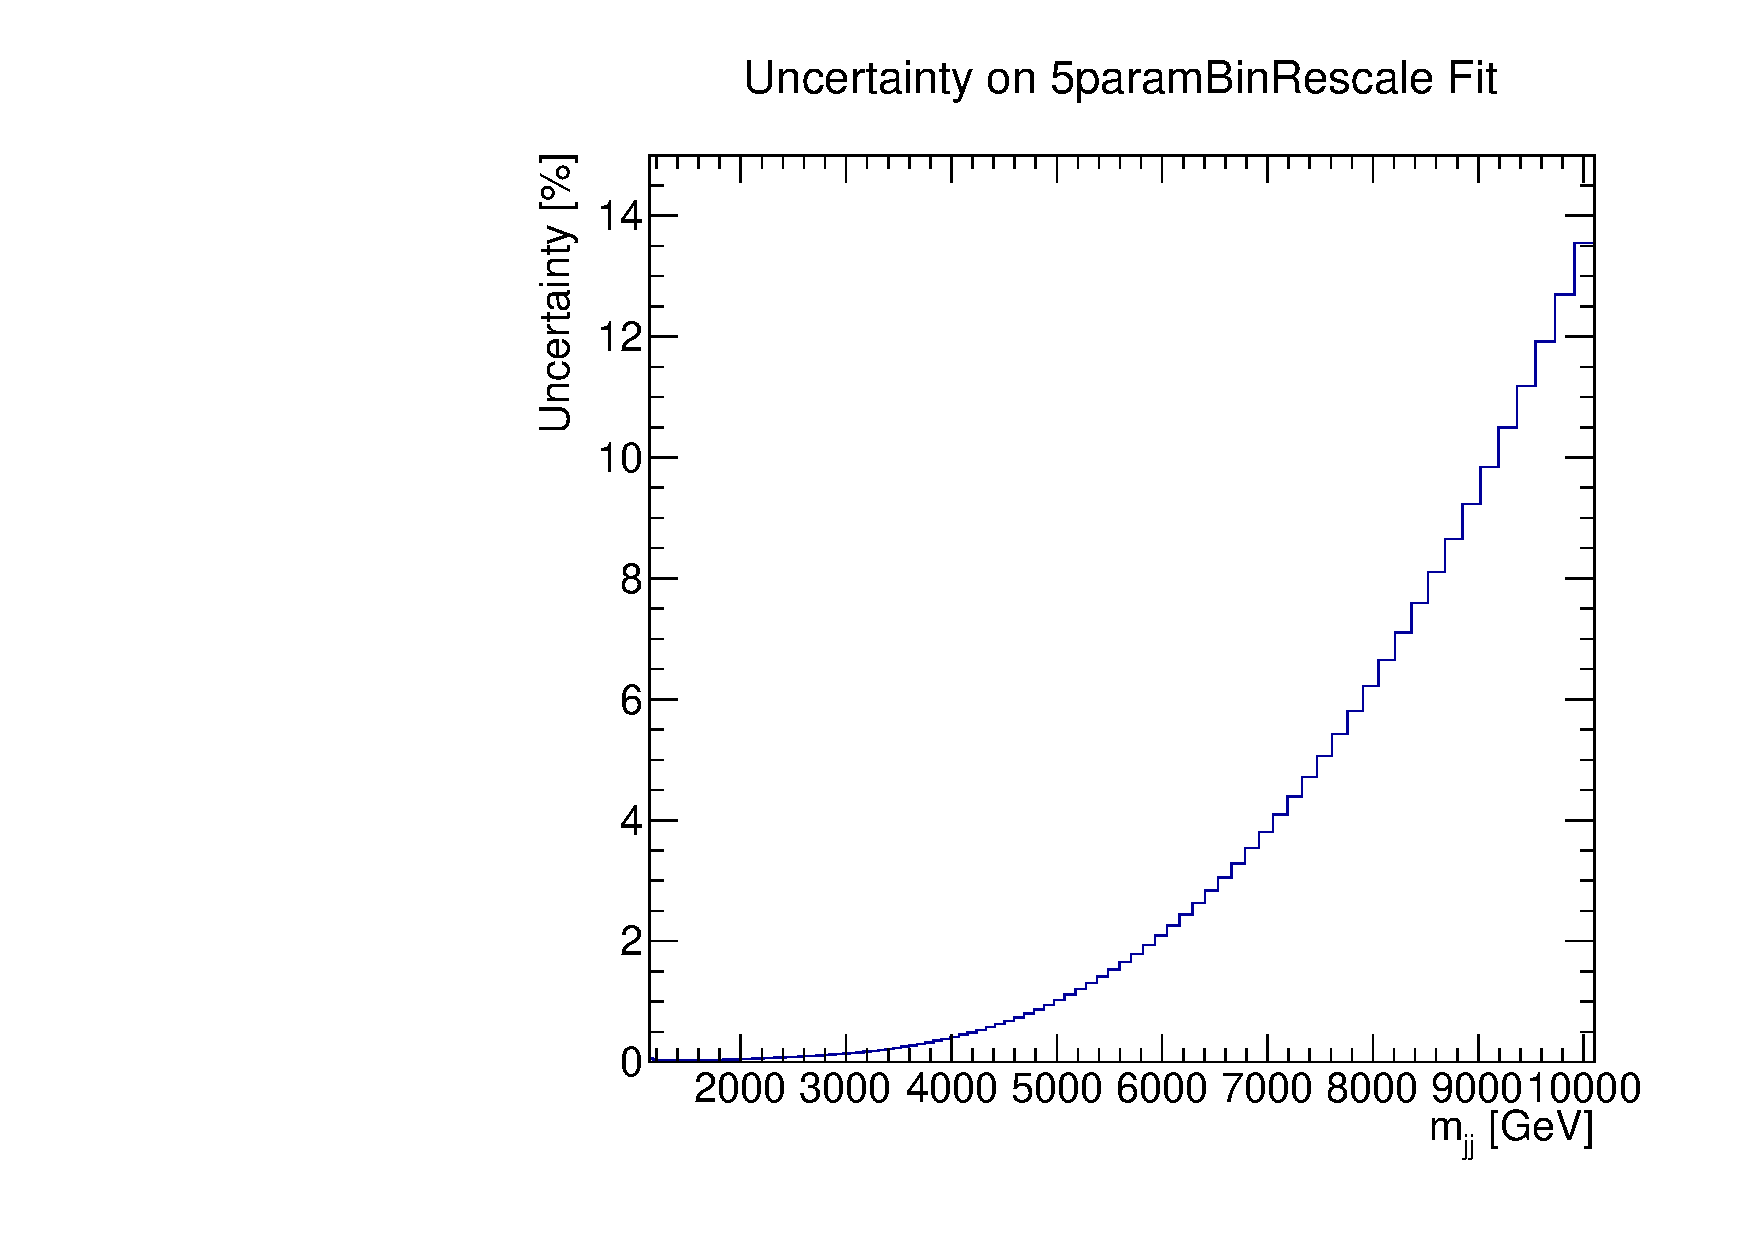
\includegraphics[width=1\linewidth]{figures/app-GlobalFitStudies/5ParamGlobalFit_ystar0.8_Uncertainty.pdf}
    \caption{Scaling per bin between a distribution rescaled by bin width to produce a plot of Events / GeV in each bin and a plot of raw events.}
    \label{fig:BinningShapeAdjustment}
\end{figure}


\begin{figure}
  \hspace{-3.3cm}
  \begin{subfigure}{.8\linewidth}
    \centering
    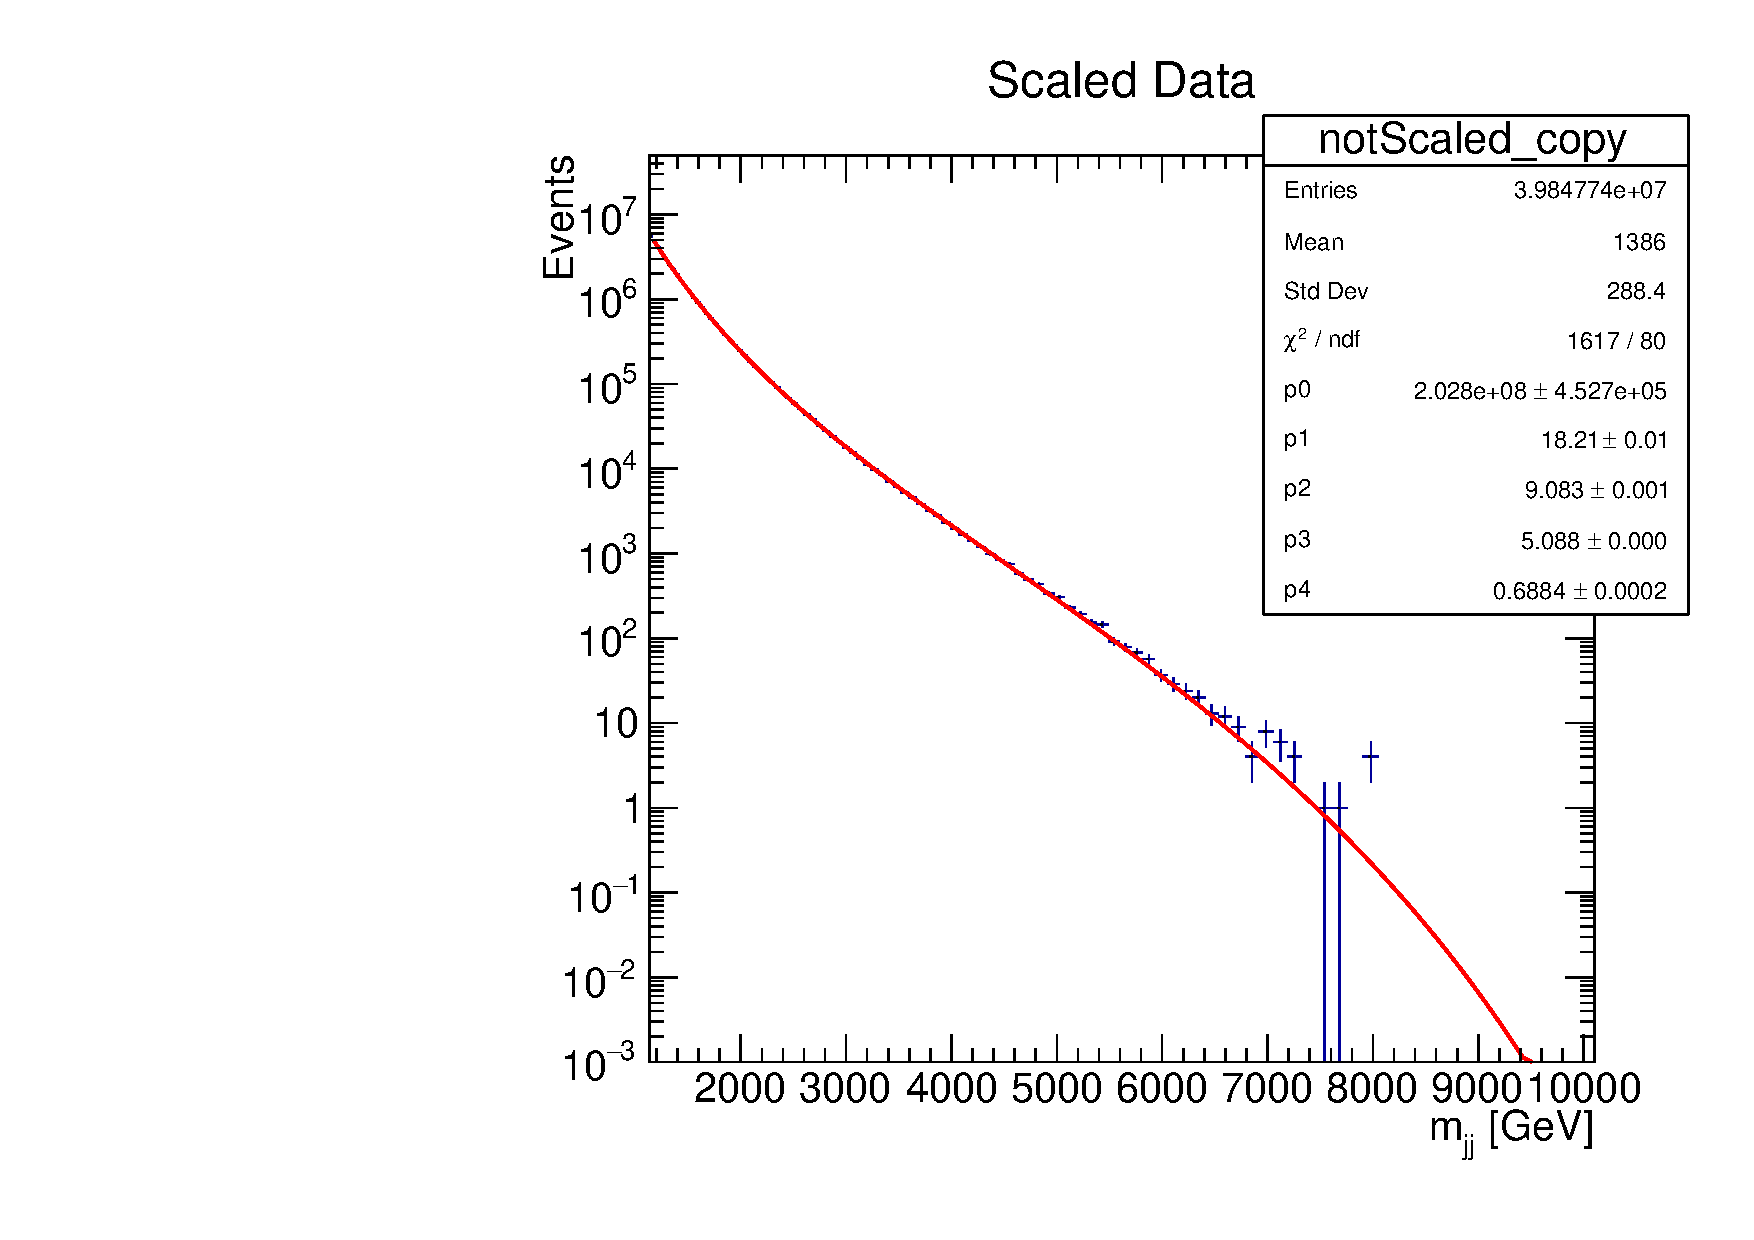
\includegraphics[width=1\linewidth]{figures/app-GlobalFitStudies/5ParamGlobalFit_ystar0.8_NoRescalingProcedure.pdf}
    \caption{Fitted events per bin}
    \label{fig:sub15ParamGlobalFitBinRescaleComparison}
  \end{subfigure}%
  \begin{subfigure}{.8\linewidth}
    \centering
    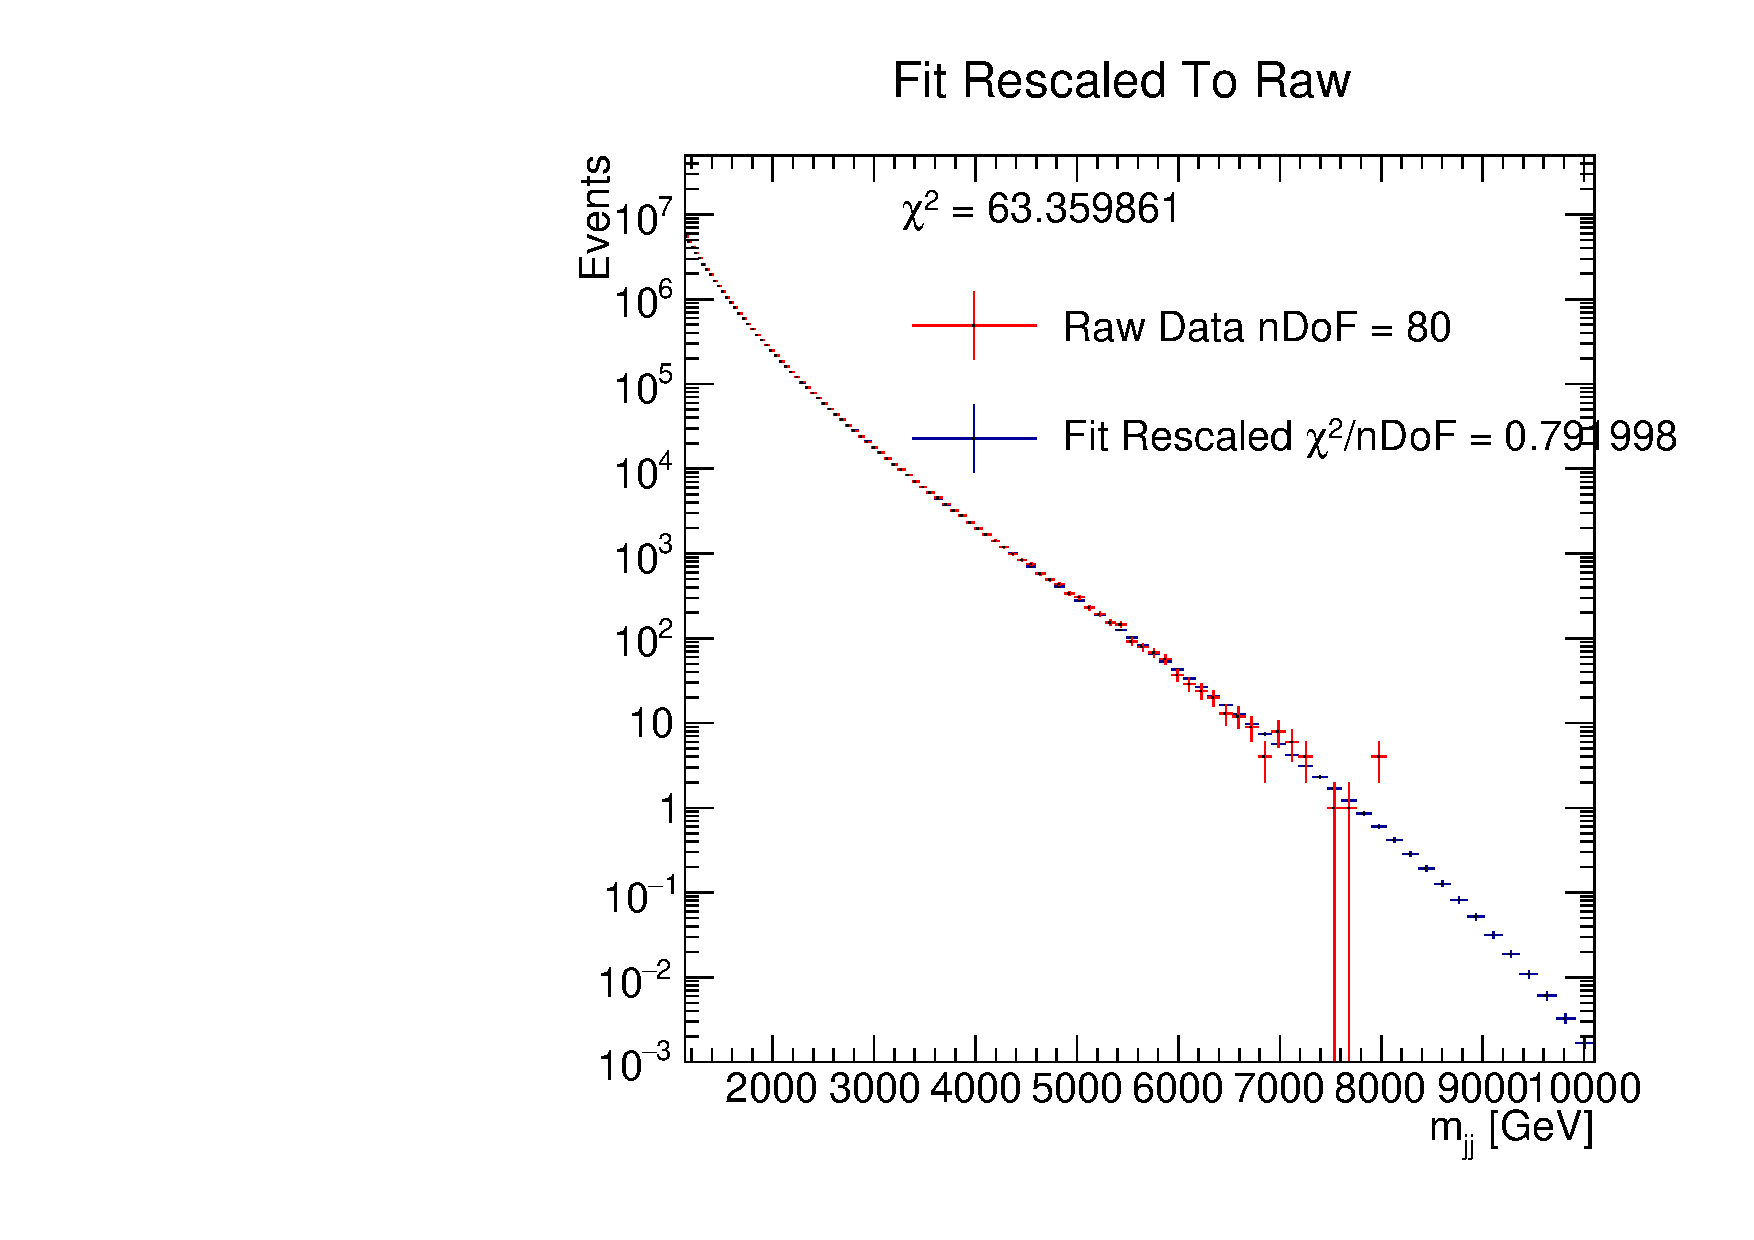
\includegraphics[width=1\linewidth]{figures/app-GlobalFitStudies/5ParamGlobalFit_ystar0.8.pdf}
    \caption{Fitted events / GeV per bin via bin rescaling procedure.}
    \label{fig:sub25ParamGlobalFitBinRescaleComparison}
  \end{subfigure}
  \caption{string resonance cuts inclusive $|y*|<0.8$ data fitted using MINUIT2 with a 5 parameter dijet fit function, both globally fitting the measured data in events per bin and performing the bin rescaling procedure. The measured $\frac{\chi^{2}}{nDoF}$ of the fit is improved via this bin rescaling procedure by a factor of 20 from 1617/80 to 63.4/80.}
  \label{fig:5ParamGlobalFitBinRescaleComparison}
\end{figure}

\subsection{Fit Statistical Uncertainty}
\label{subsec:fitStatUnc:GlobalFitting}

To estimate the $1\sigma$ statistical uncertainty upon the fit, a pseudo-experiment method is used, which has been used in many other analyses including the previous dijet analysis \cite{ATL-COM-PHYS-2018-1538}.

\begin{itemize}
    \item A large number (10,000 or more) of pseudoexperiments are generated, generated by pulling from a poisson distribution at each bin of the nominal fit with mean set to equal the bin.
    \item Each pseudoexperiment is fit with the bin rescaling procedure, with initial fit parameters set to the value of the nominal fit.
    \item the RMS of all pseudoexperiments in each bin is calculated and set as the statistical uncertainty.
\end{itemize}

The statistical uncertainty on the 5 parameter dijet fit function globally fitted using MINUIT2 on data with string resonance cuts after performing this procedure is shown in Figure \ref{fig:5ParamStatisticalUncertainty}, with a statistical uncertainty $ < $ 6.2\% up to 8 TeV. Statistical uncertainties of additional fit functions are available in \\ {\href{https://indico.cern.ch/event/997813/contributions/4191921/attachments/2178521/3679266/dijet_CompareBinRescale_26_01_2021.pdf}{https://indico.cern.ch/event/997813/contributions/4191921/}}.

\begin{figure}
    \centering
    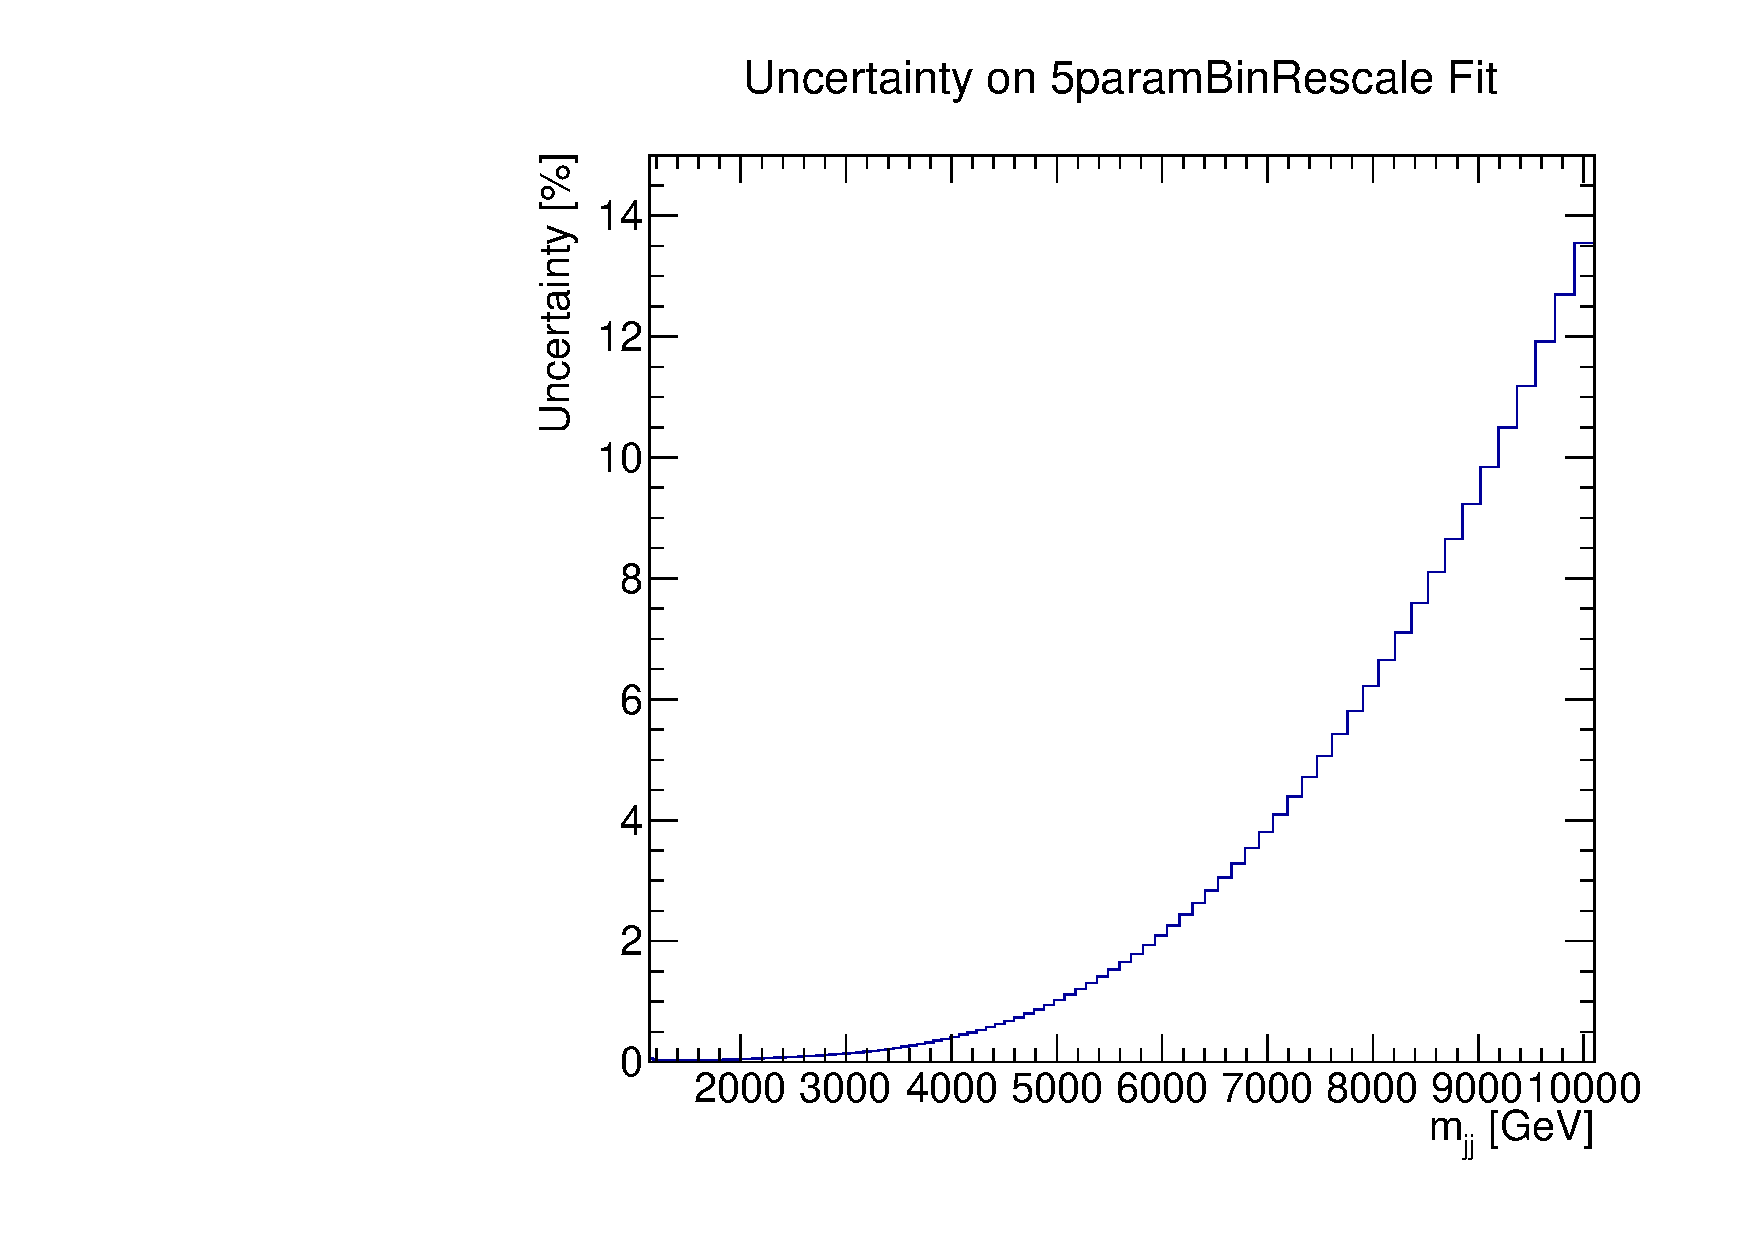
\includegraphics[width=1\linewidth]{figures/app-GlobalFitStudies/5ParamGlobalFit_ystar0.8_Uncertainty.pdf}
    \caption{Statistical uncertainty on a 5 parameter dijet fit function fit using MINUIT2 with string resonance cuts to inclusive $|y*|<0.8$ data.}
    \label{fig:5ParamStatisticalUncertainty}
\end{figure}

\subsection{Choice of Minimizer}
\label{subsec:MinimizerChoice:GlobalFitting}
The MINUIT2 minimizer is used as standard, the statistical uncertainty of the 5 parameter dijet fit function globally fitted on data with string resonance cuts obtained with MINUIT2 in comparison to MINUIT is shown in Figure \ref{fig:5ParamMINUITComparison}, showing that MINUIT has a statistical uncertainty $ < $ 9\% up to 8 TeV, $\approx$ 3\% larger at 8 TeV than the MINUIT2 case.

\begin{figure}
    \centering
    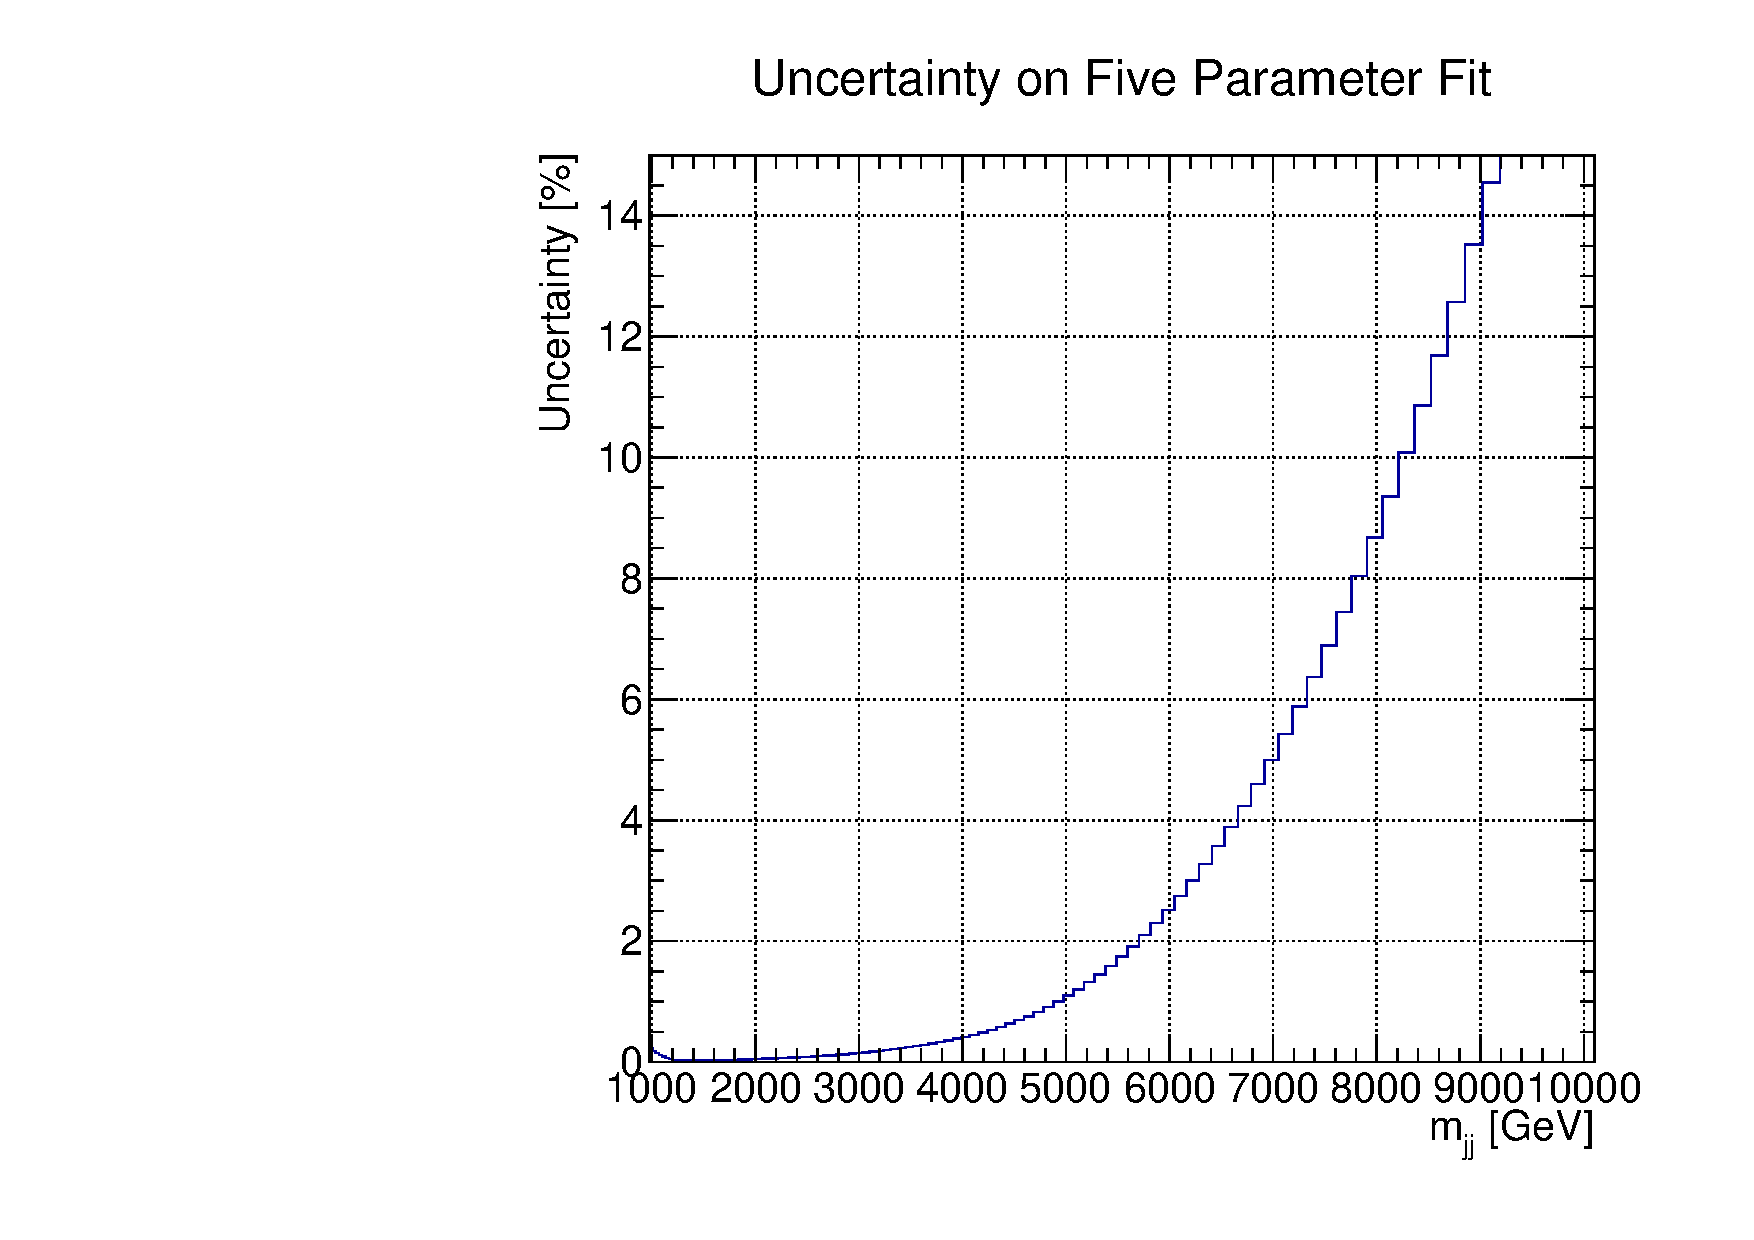
\includegraphics[width=1\linewidth]{figures/app-GlobalFitStudies/5ParamGlobalFit_ystar0.8_Uncertainty_MINUIT.pdf}
    \caption{Statistical uncertainty on a 5 parameter dijet fit function global fit using MINUIT with string resonance cuts to inclusive $|y*|<0.8$ data.}
    \label{fig:5ParamMINUITComparison}
\end{figure}


\subsection{SWiFt Vs Global Fitting}
\label{subsec:SWiFtVsGlobal:GlobalFitting}

The statistical uncertainty found on the fit using SWiFt instead of global fitting is shown in Figure \ref{fig:SWiFtStatisticalUncertaintyYstar0.8}, with a statistical uncertainty of $ < $ 44\% up to 8 TeV, $\approx$ 38\% larger at 8 TeV than the global fitting case. Due to this increased statistical uncertainty and also due to the inherent simplicity of global fits allowing easier reinterpretation by theorists, using the global fit rather than SWiFt fit is motivated.

\begin{figure}
    \centering
    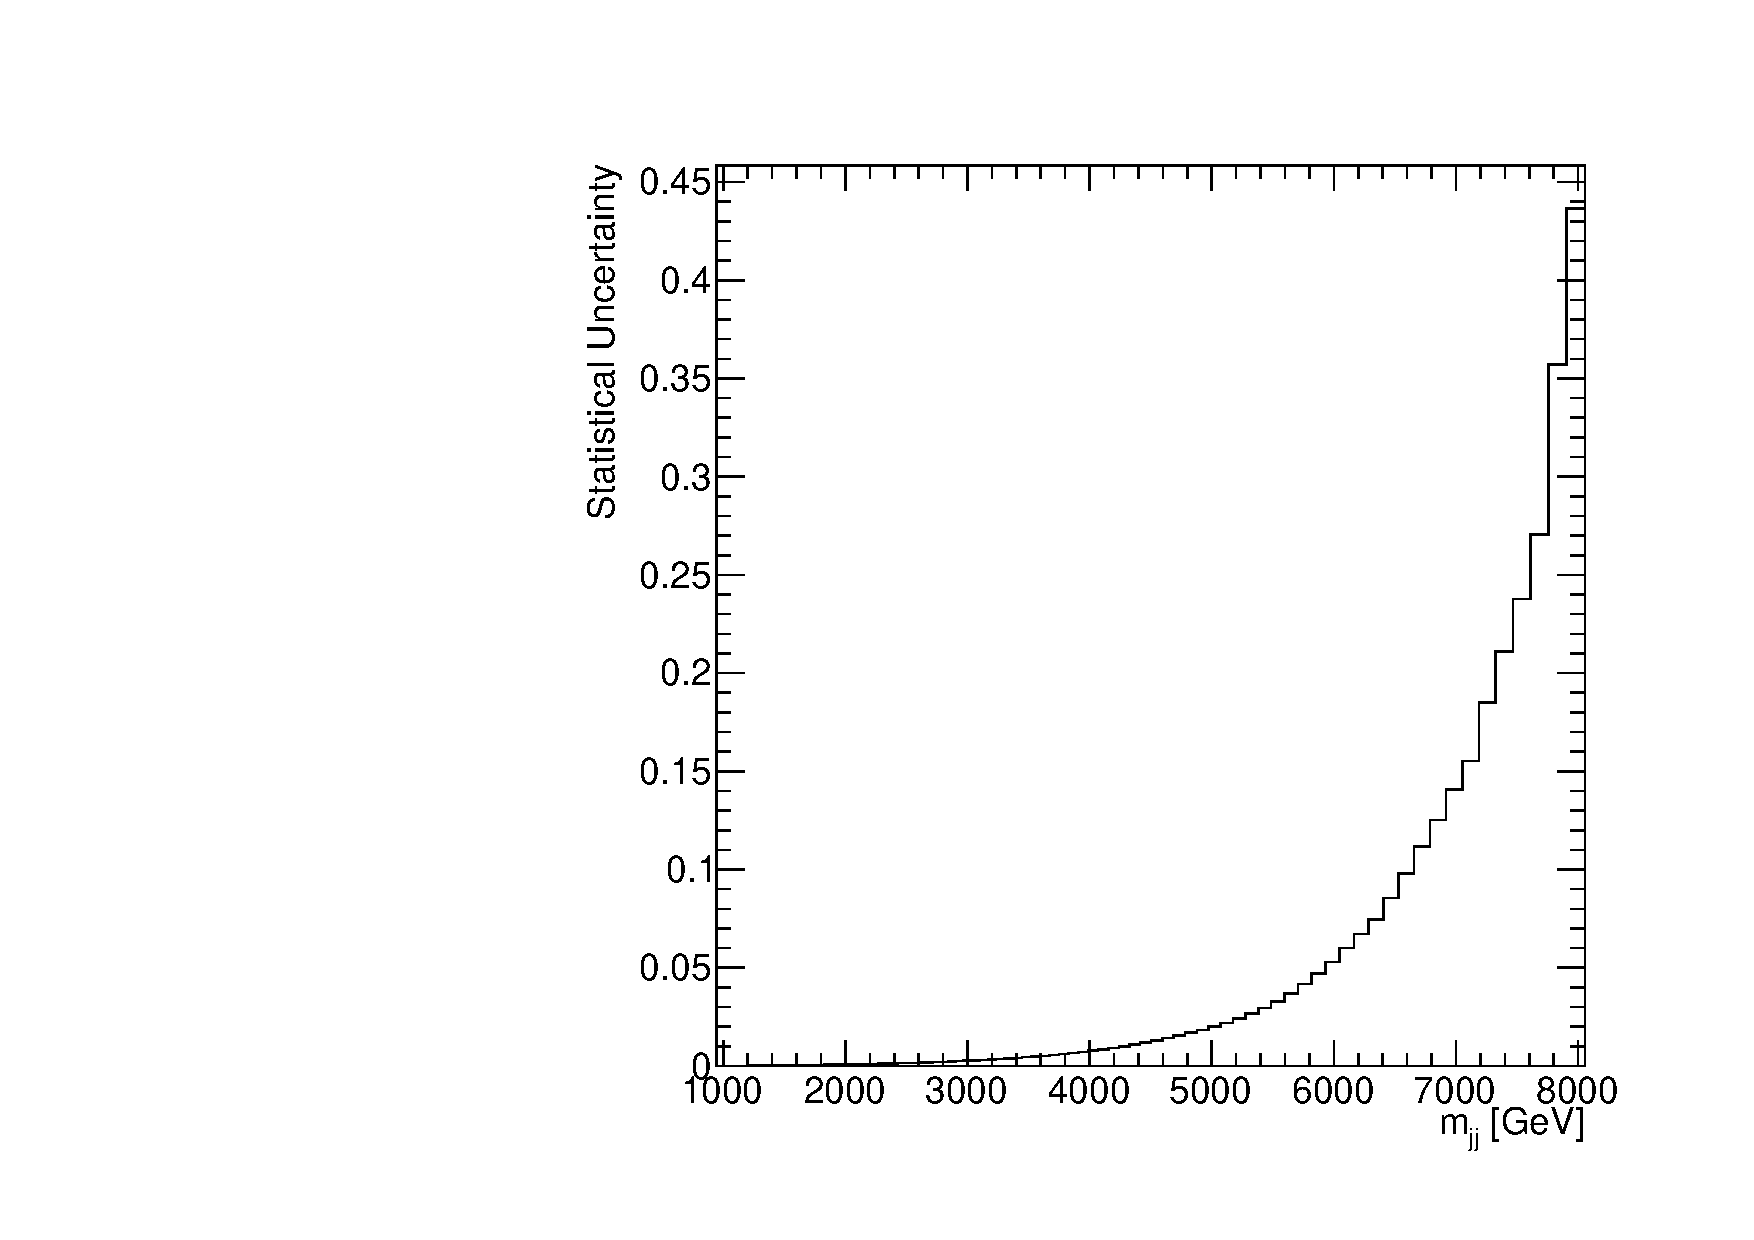
\includegraphics[width=1.0\linewidth]{figures/app-GlobalFitStudies/5ParamSWiFtFit_ystar0.8_Uncertainty.pdf}
    \caption{Statistical uncertainty on a 5 parameter dijet fit function SWiFt fit with string resonance cuts to inclusive $|y*|<0.8$ data.}
    \label{fig:SWiFtStatisticalUncertaintyYstar0.8}
\end{figure}

\subsubsection{Bump Hunter}
\label{subsubsec:BH:GlobalFitting}

The significance per bin was calculated using BumpHunter both using SWiFt and global fitting for string resonance cuts to inclusive $|y*|<0.8$ data in Figure \ref{fig:ystar0.8FullRunBHFits}, the BumpHunter p-value for these is shown in Figure \ref{fig:ystar0.8FullRunBHPvalue}, showing both SWiFt and global fitting produce consistent significance plots and p-values for this region (0.93 vs 0.90 respectively).

The same was done using instead the H' cuts with $|y*|<0.6$, significance shown in Figure \ref{fig:ystar0.6FullRunBHFits} and p-value shown in Figure \ref{fig:ystar0.6FullRunBHPvalue}. It was found in the significance plot that the significance per bin at low $m_{jj}$ is consistent between SWiFt and global fitting, however at high $m_{jj}$ $\gtrsim$ TeV the significance per bin is found to be significantly larger in the global fitting case than SWiFt which results in the p-value of SWiFt being significantly higher than with global fitting (0.89 vs 0.34 respectively).

This same procedure was performed for each individual year of running (2015,2016,2017,2018), producing the fits shown in Figure \ref{fig:ystar0.6IndividualFits}, showing that the fits per year are more consistent especially at high $m_{jj}$ in the global fitting case than the SWiFt case, as expected due to the lower statistical uncertainty in the fit which explains the larger significances with global fitting in the higher $m_{jj}$ bins, as the SWiFt fit varies per year, neglecting 2015 which has too low statistics for meaningful comparison, around the 8 TeV region by as large as $\approx$ 70\%, while the global fit only varies by $\approx 5\%$. Hence, the lower significance in this region in the SWiFt case is due to the larger statistical uncertainty in the SWiFt fit, and the global fit significance for these bins is more reliable.


\begin{figure}
  \hspace{-3.3cm}
  \begin{subfigure}{.8\linewidth}
    \centering
    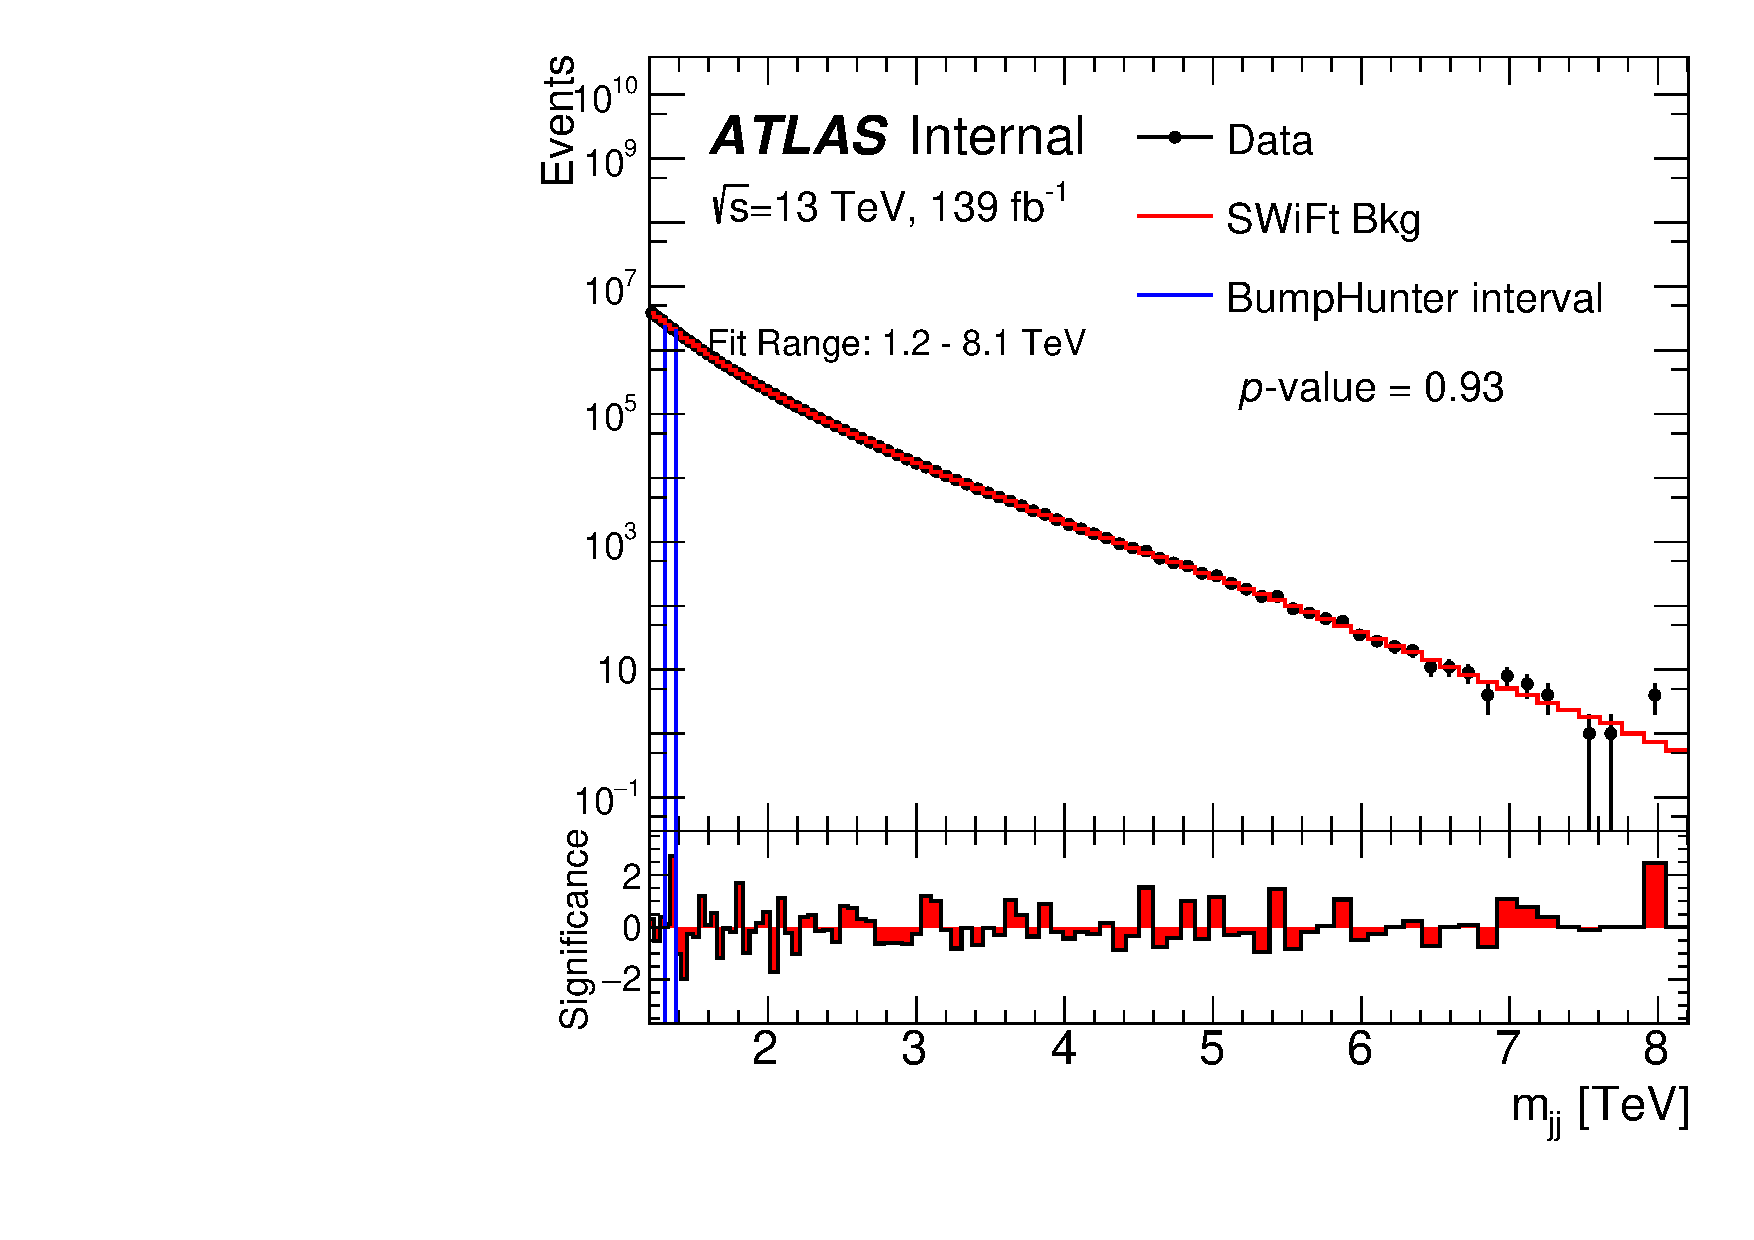
\includegraphics[width=1\linewidth,height=7cm]{figures/app-GlobalFitStudies/5ParamSwiftYStar0.8_BumpHunterSignifcance.pdf}
    \caption{SWiFt background fit}
    \label{fig:sub1ystar0.8FullRunBHFits}
  \end{subfigure}%
  \begin{subfigure}{.8\linewidth}
    \centering
    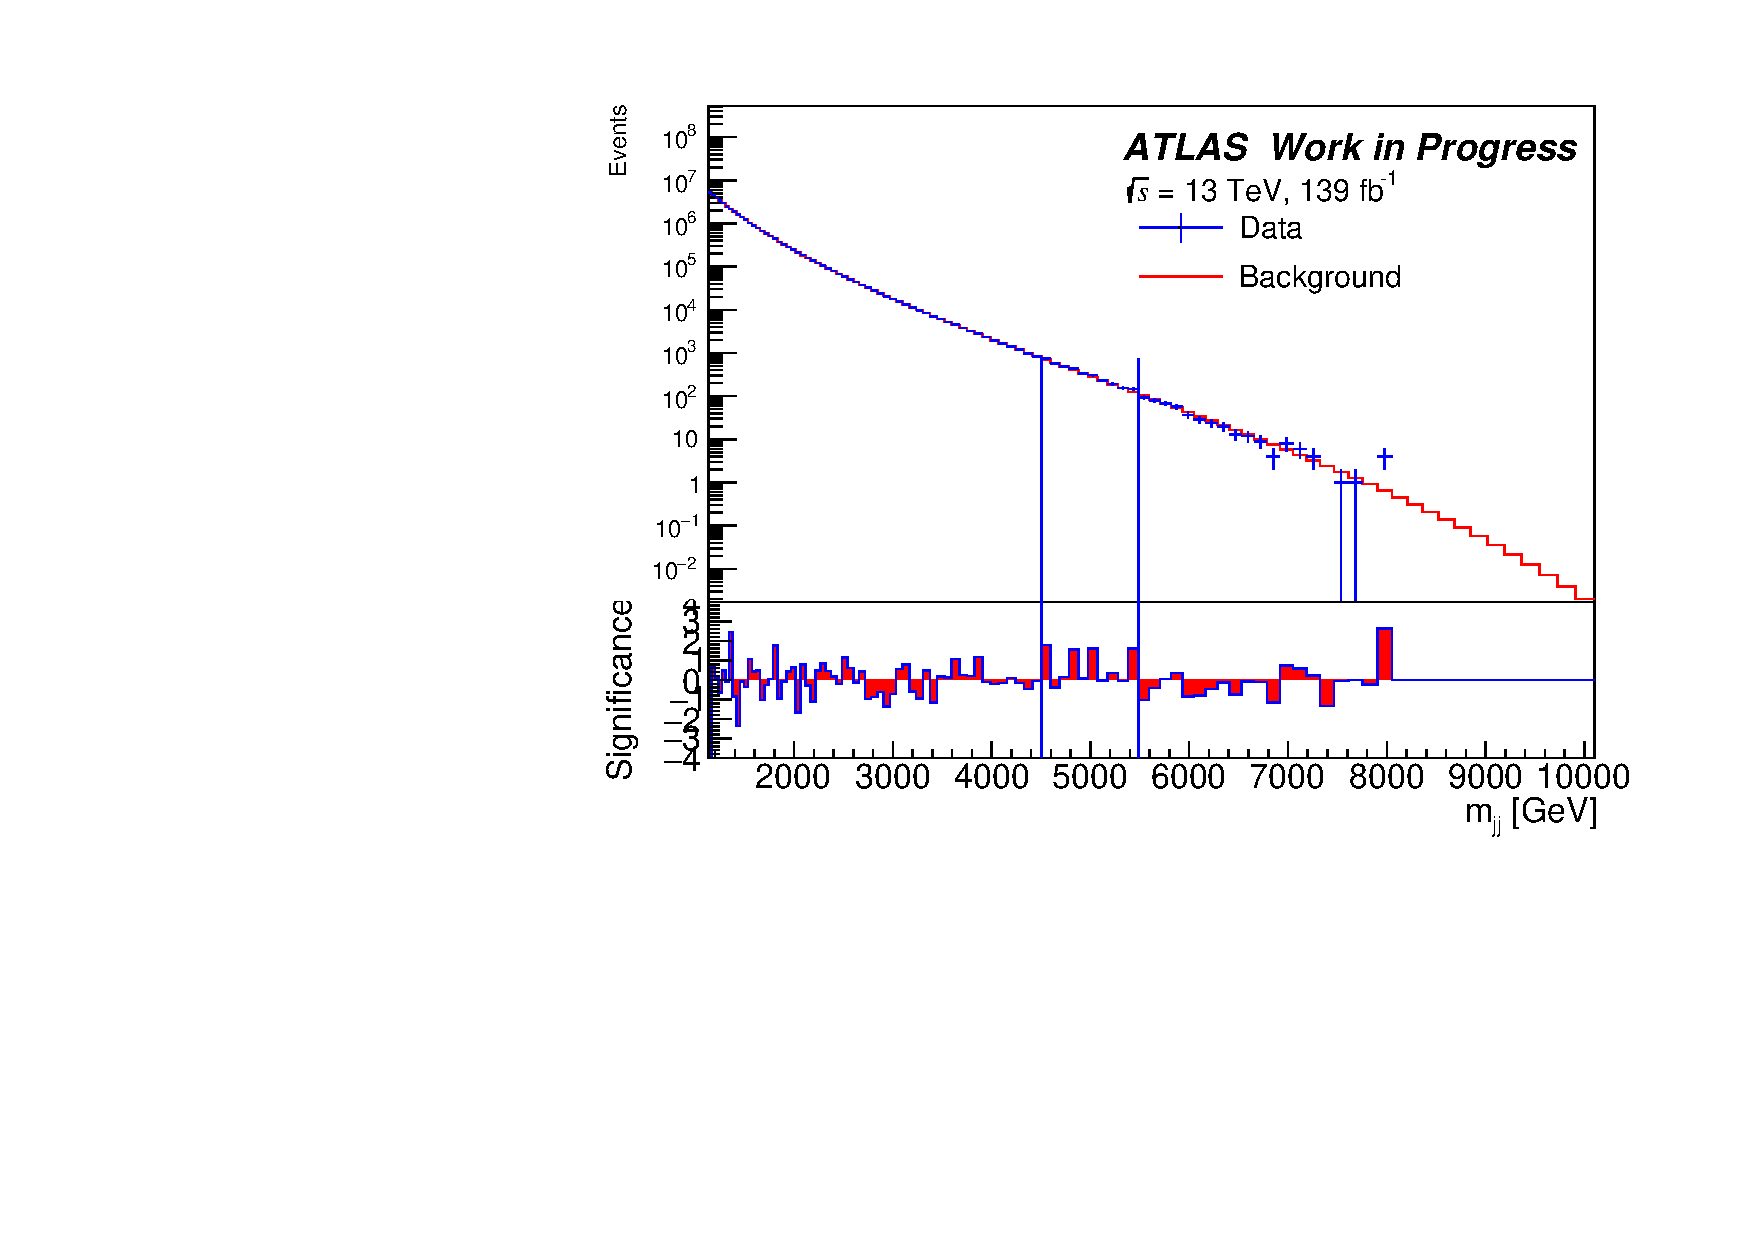
\includegraphics[trim=35 2 10 30, clip,width=1.1\linewidth,height=7cm]{figures/app-GlobalFitStudies/5ParamGlobalYStar0.8_BumpHunterSignifcance.pdf}
    \caption{Global background fit}
    \label{fig:sub2ystar0.8FullRunBHFits}
  \end{subfigure}
  \caption{significance per bin calculated using BumpHunter for string resonance cuts inclusive $|y*|<0.8$ data fitted with a 5 parameter dijet fit function fitted both with SWiFt and globally, showing consistent significance plots between SWiFt and global fitting.}
  \label{fig:ystar0.8FullRunBHFits}
\end{figure}


\begin{figure}
  \hspace{-3.3cm}
  \begin{subfigure}{.8\linewidth}
    \centering
    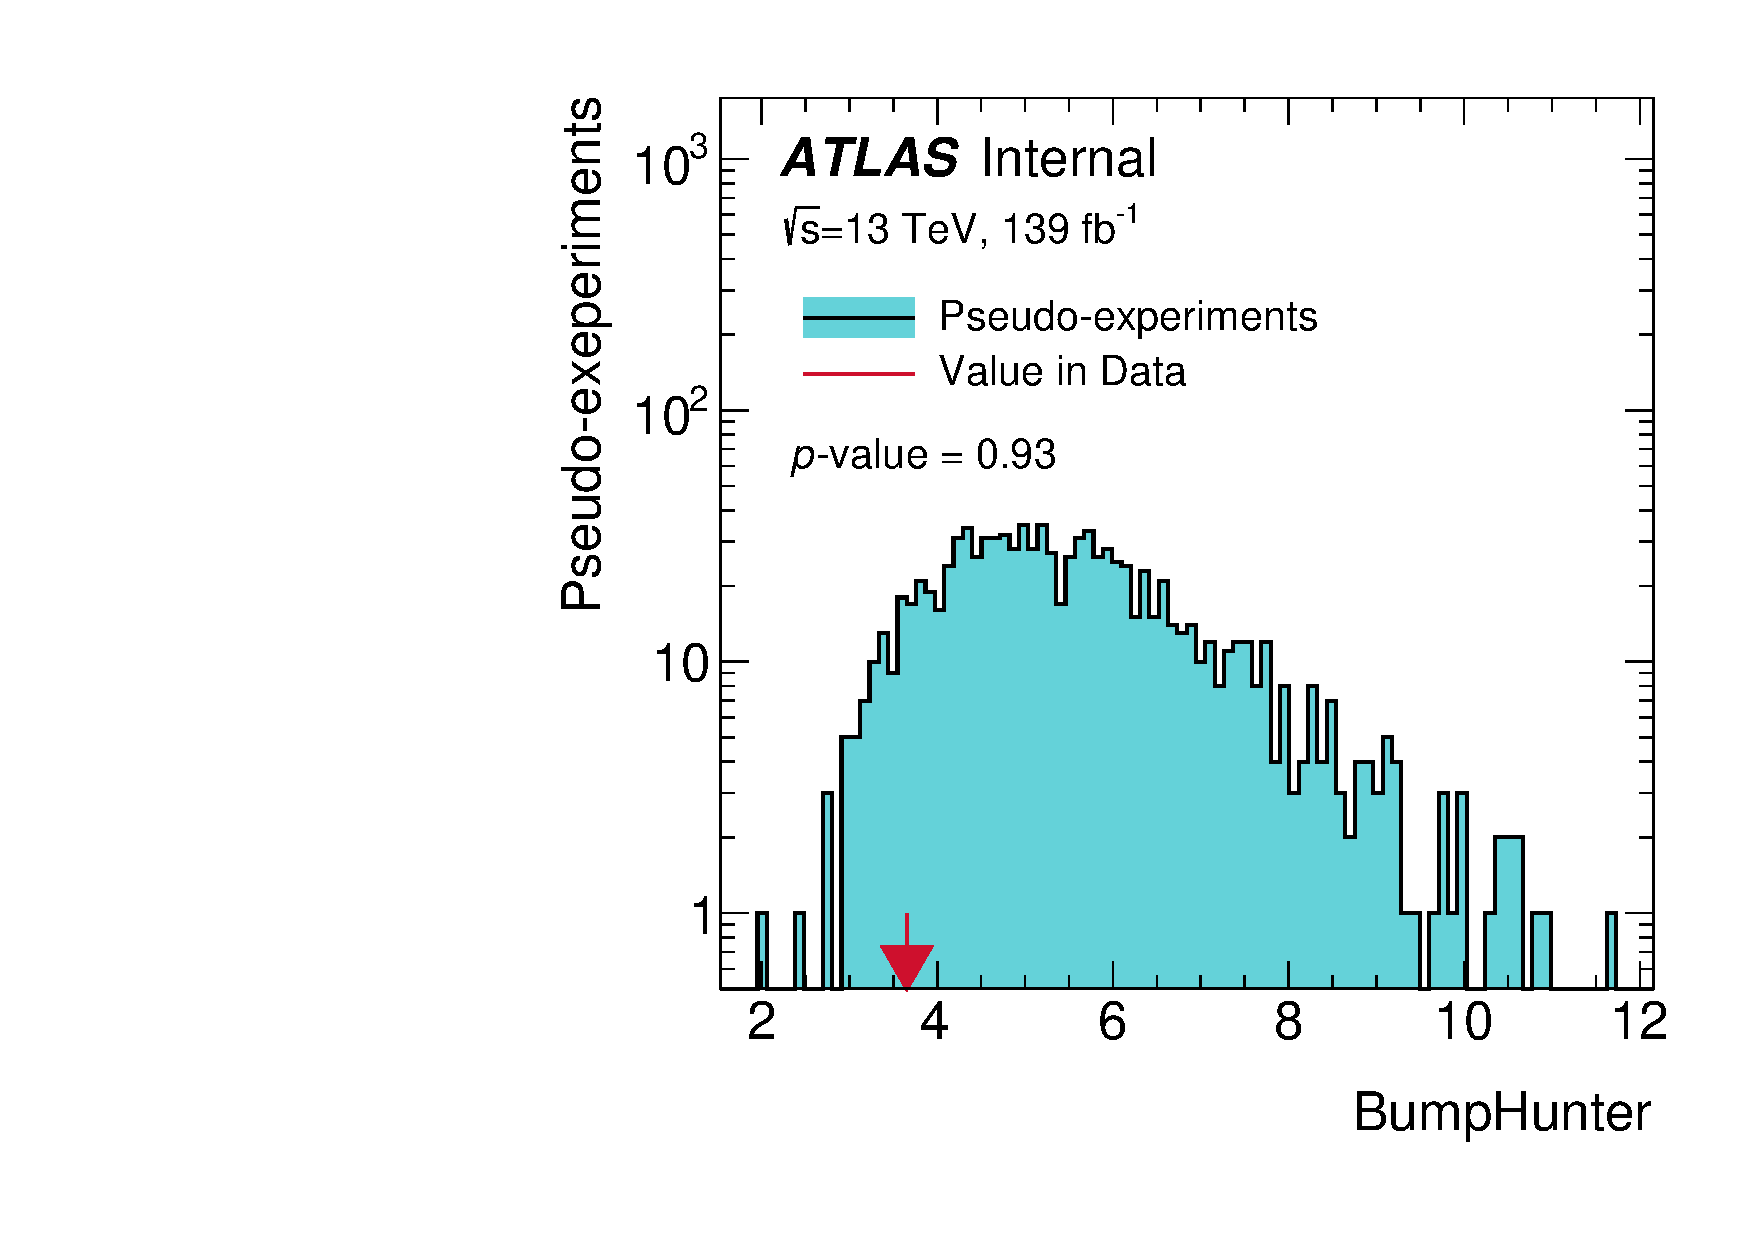
\includegraphics[trim=0 0 0 20, clip,width=1.0\linewidth,height=6cm]{figures/app-GlobalFitStudies/5ParamSwiftYStar0.8_BumpHunterPValue.pdf}
    \label{fig:sub1ystar0.8FullRunBHPvalue}
  \end{subfigure}%
  \begin{subfigure}{.8\linewidth}
    \centering
    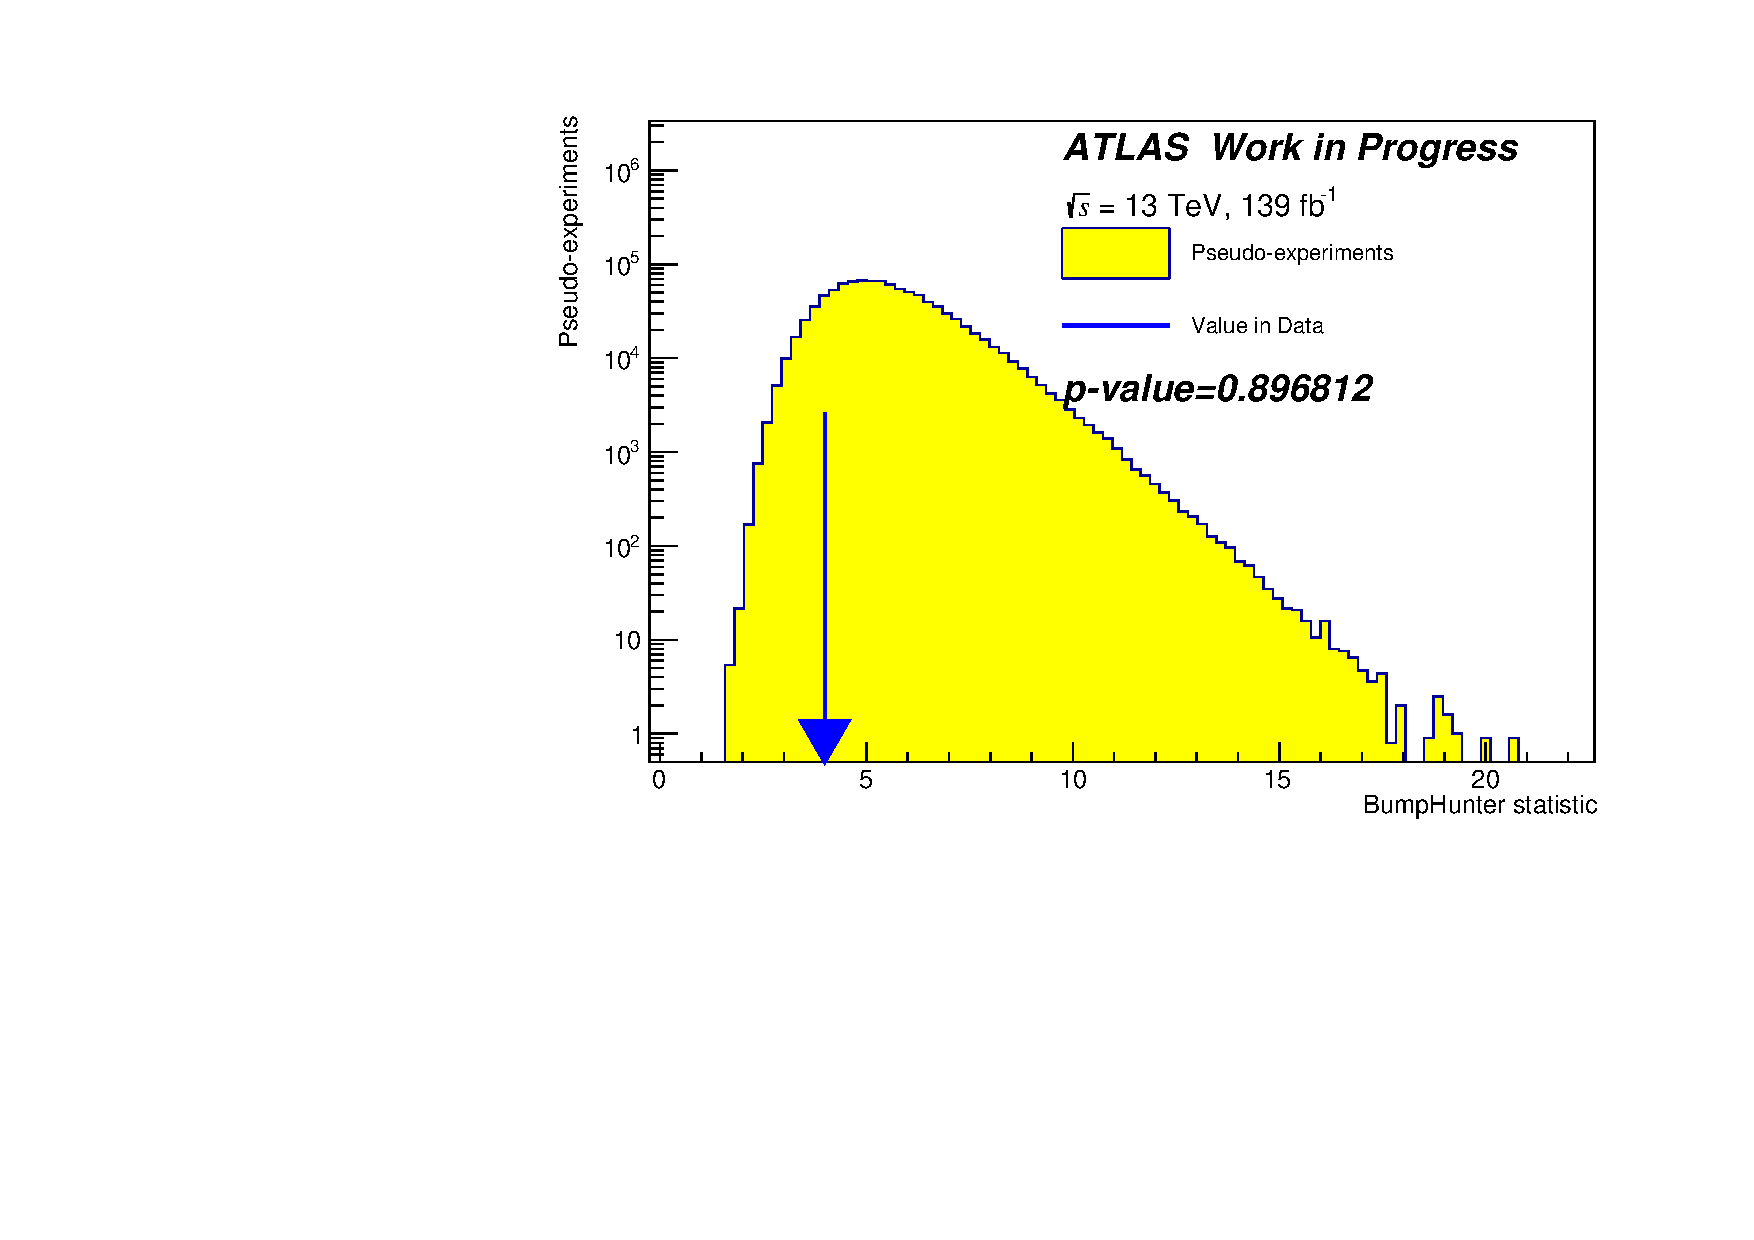
\includegraphics[trim=10 2 35 35, clip,width=1.0\linewidth,height=6cm]{figures/app-GlobalFitStudies/5ParamGlobalYStar0.8_BumpHunterPValue.pdf}
    \caption{Global background fit}
    \label{fig:sub2ystar0.8FullRunBHPvalue}
  \end{subfigure}
  \caption{BumpHunter p-values calculated using BumpHunter for string resonance cuts inclusive $|y*|<0.8$ data fitted with a 5 parameter dijet fit function fitted both with SWiFt and globally, showing consistent p-values between SWiFt and global fitting.}
  \label{fig:ystar0.8FullRunBHPvalue}
\end{figure}


\begin{figure}
  \hspace{-3.3cm}
  \begin{subfigure}{.8\linewidth}
    \centering
    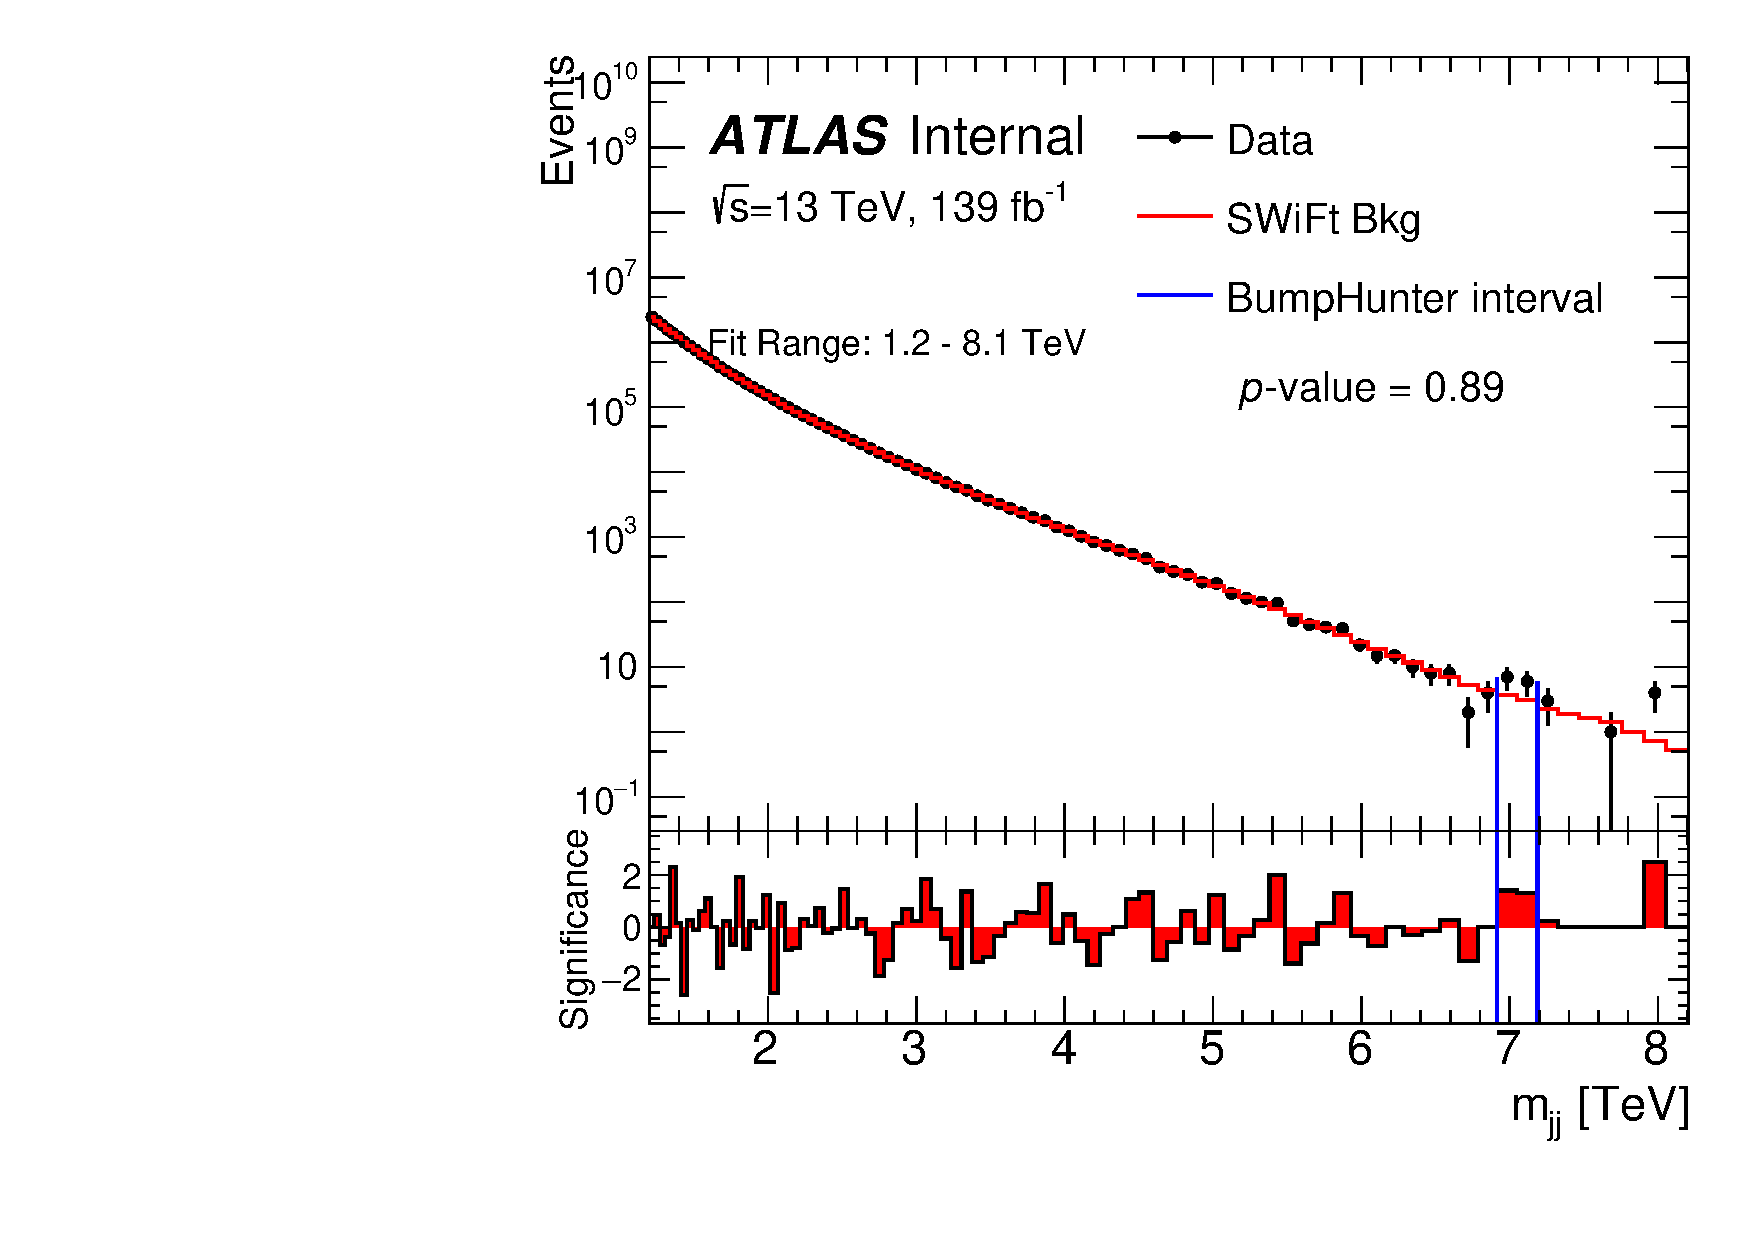
\includegraphics[width=1\linewidth,height=7cm]{figures/app-GlobalFitStudies/5ParamSwiftYStar0.6_BumpHunterSignifcance.pdf}
    \caption{SWiFt background fit}
    \label{fig:sub1ystar0.6FullRunBHFits}
  \end{subfigure}%
  \begin{subfigure}{.8\linewidth}
    \centering
    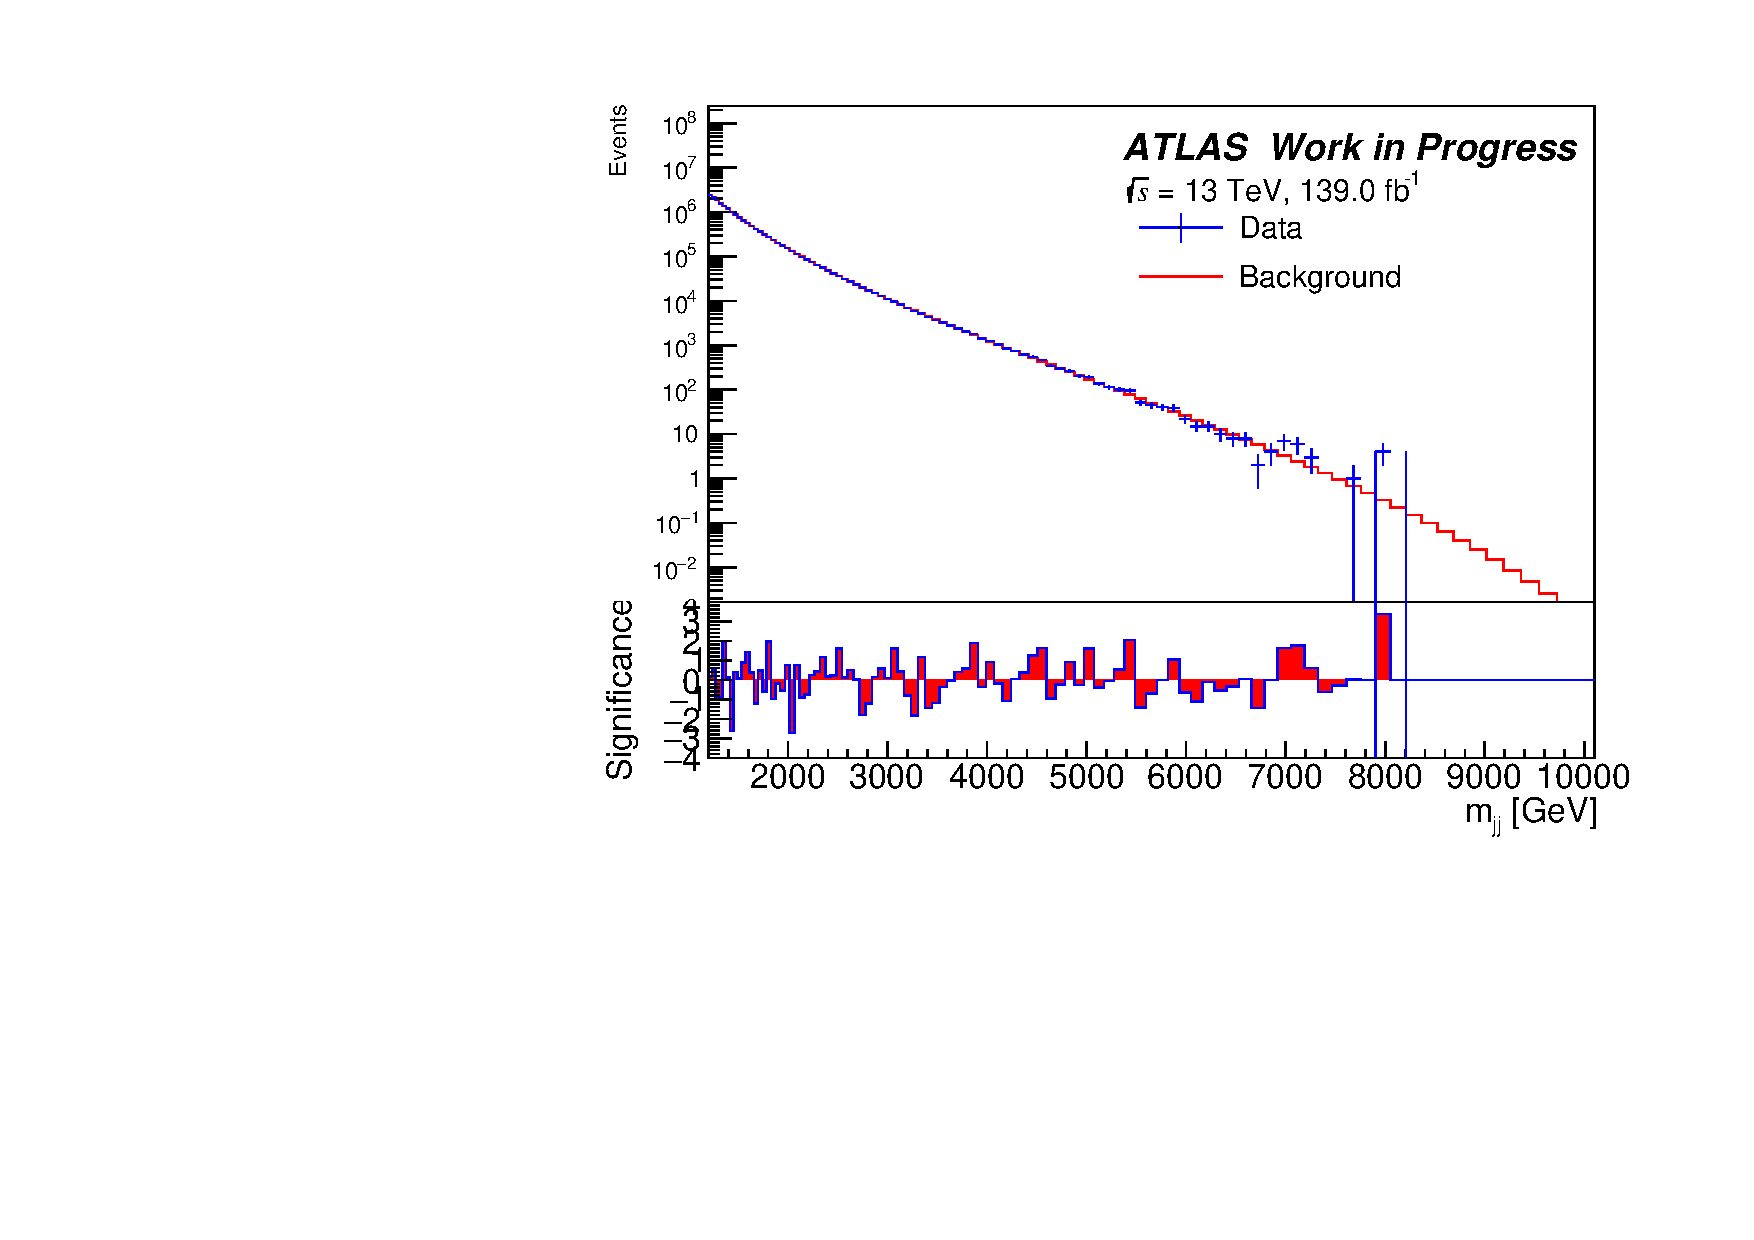
\includegraphics[trim=35 2 10 30, clip,width=1.1\linewidth,height=7cm]{figures/app-GlobalFitStudies/5ParamGlobalYStar0.6_BumpHunterSignifcance.pdf}
    \caption{Global background fit}
    \label{fig:sub2ystar0.6FullRunBHFits}
  \end{subfigure}
  \caption{significance per bin calculated using BumpHunter for H' cuts inclusive $|y*|<0.6$ data fitted with a 5 parameter dijet fit function fitted both with SWiFt and globally, showing consistent significance plots between SWiFt and global fitting at low $m_{jj}$, but significantly larger significances are observed in the global fit at high $m_{jj}$.}
  \label{fig:ystar0.6FullRunBHFits}
\end{figure}


\begin{figure}
  \hspace{-3.3cm}
  \begin{subfigure}{.8\linewidth}
    \centering
    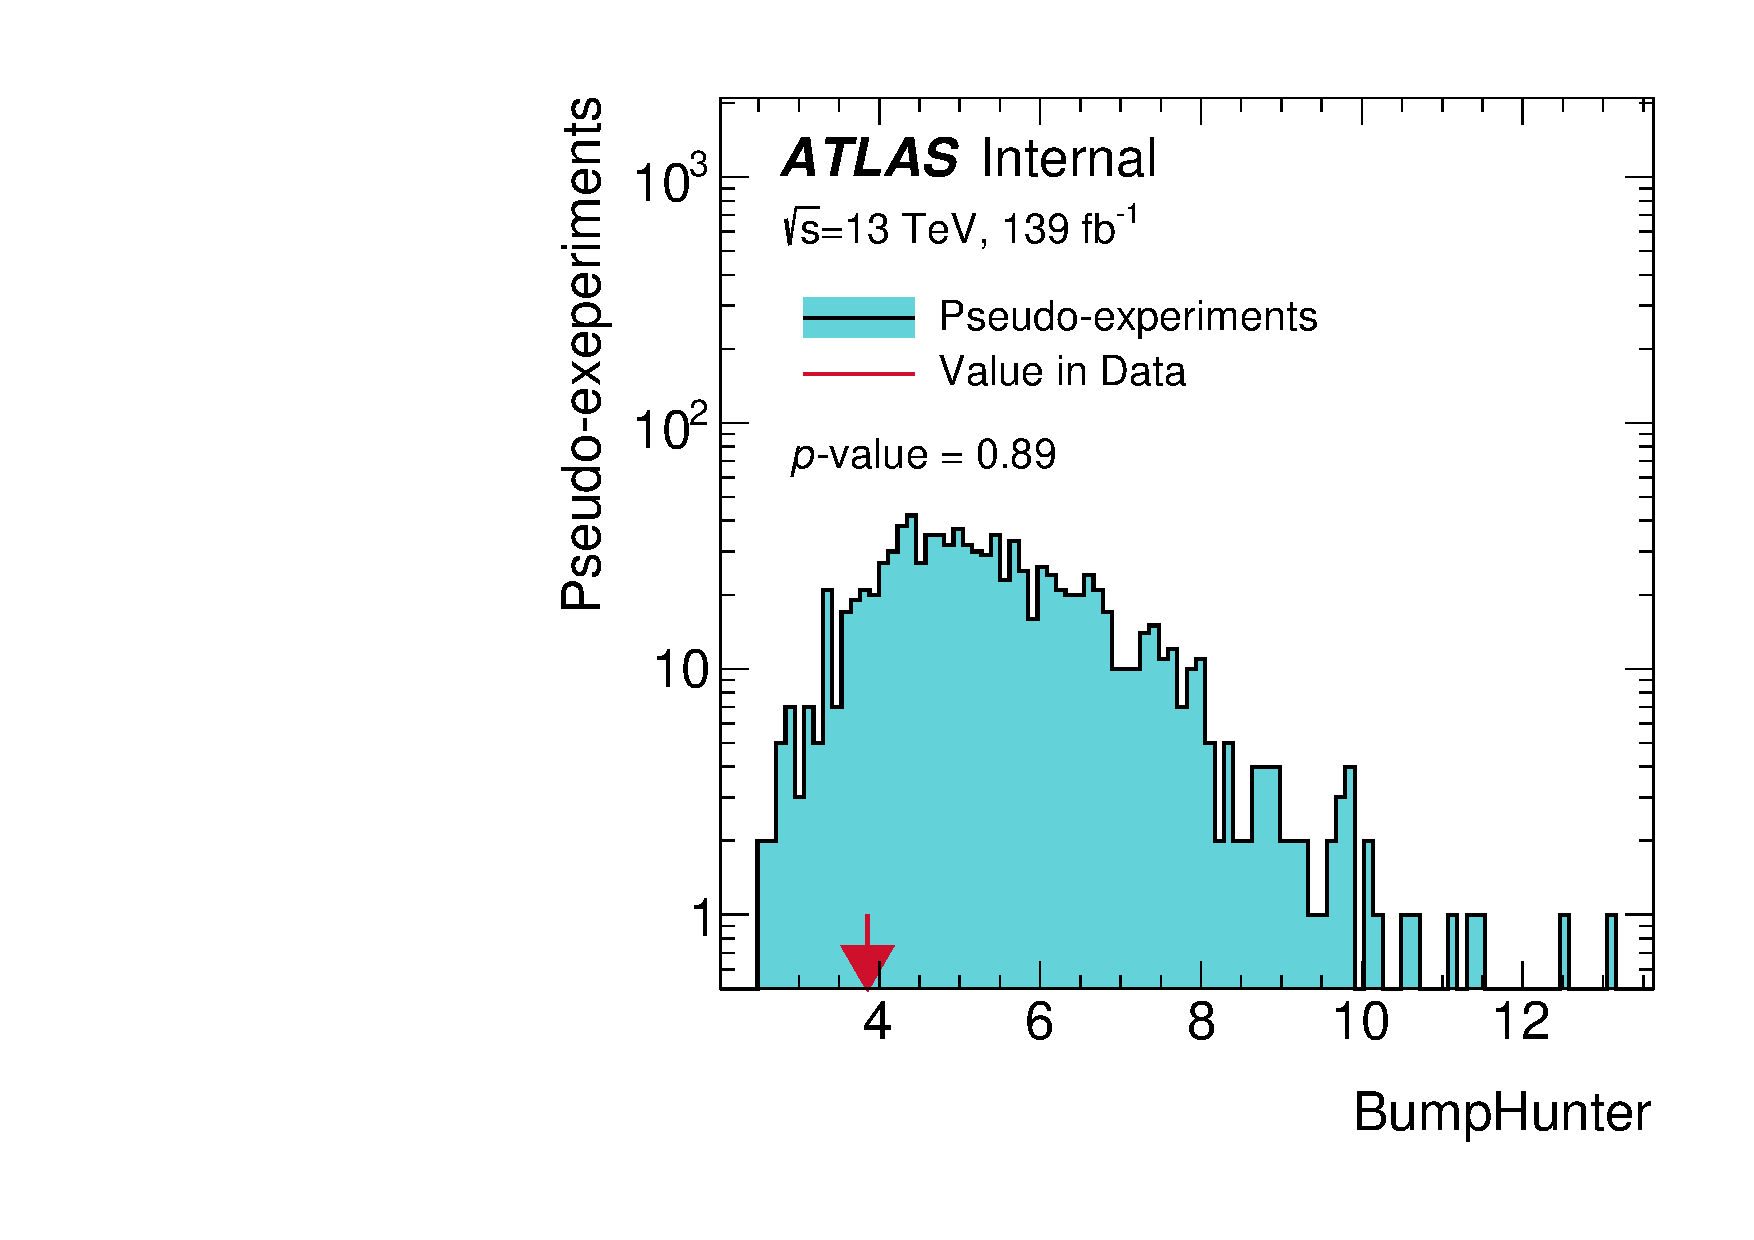
\includegraphics[trim=0 0 0 20, clip,width=1.0\linewidth,height=6cm]{figures/app-GlobalFitStudies/5ParamSwiftYStar0.6_BumpHunterPValue.pdf}
    \label{fig:sub1ystar0.6FullRunBHPvalue}
  \end{subfigure}%
  \begin{subfigure}{.8\linewidth}
    \centering
    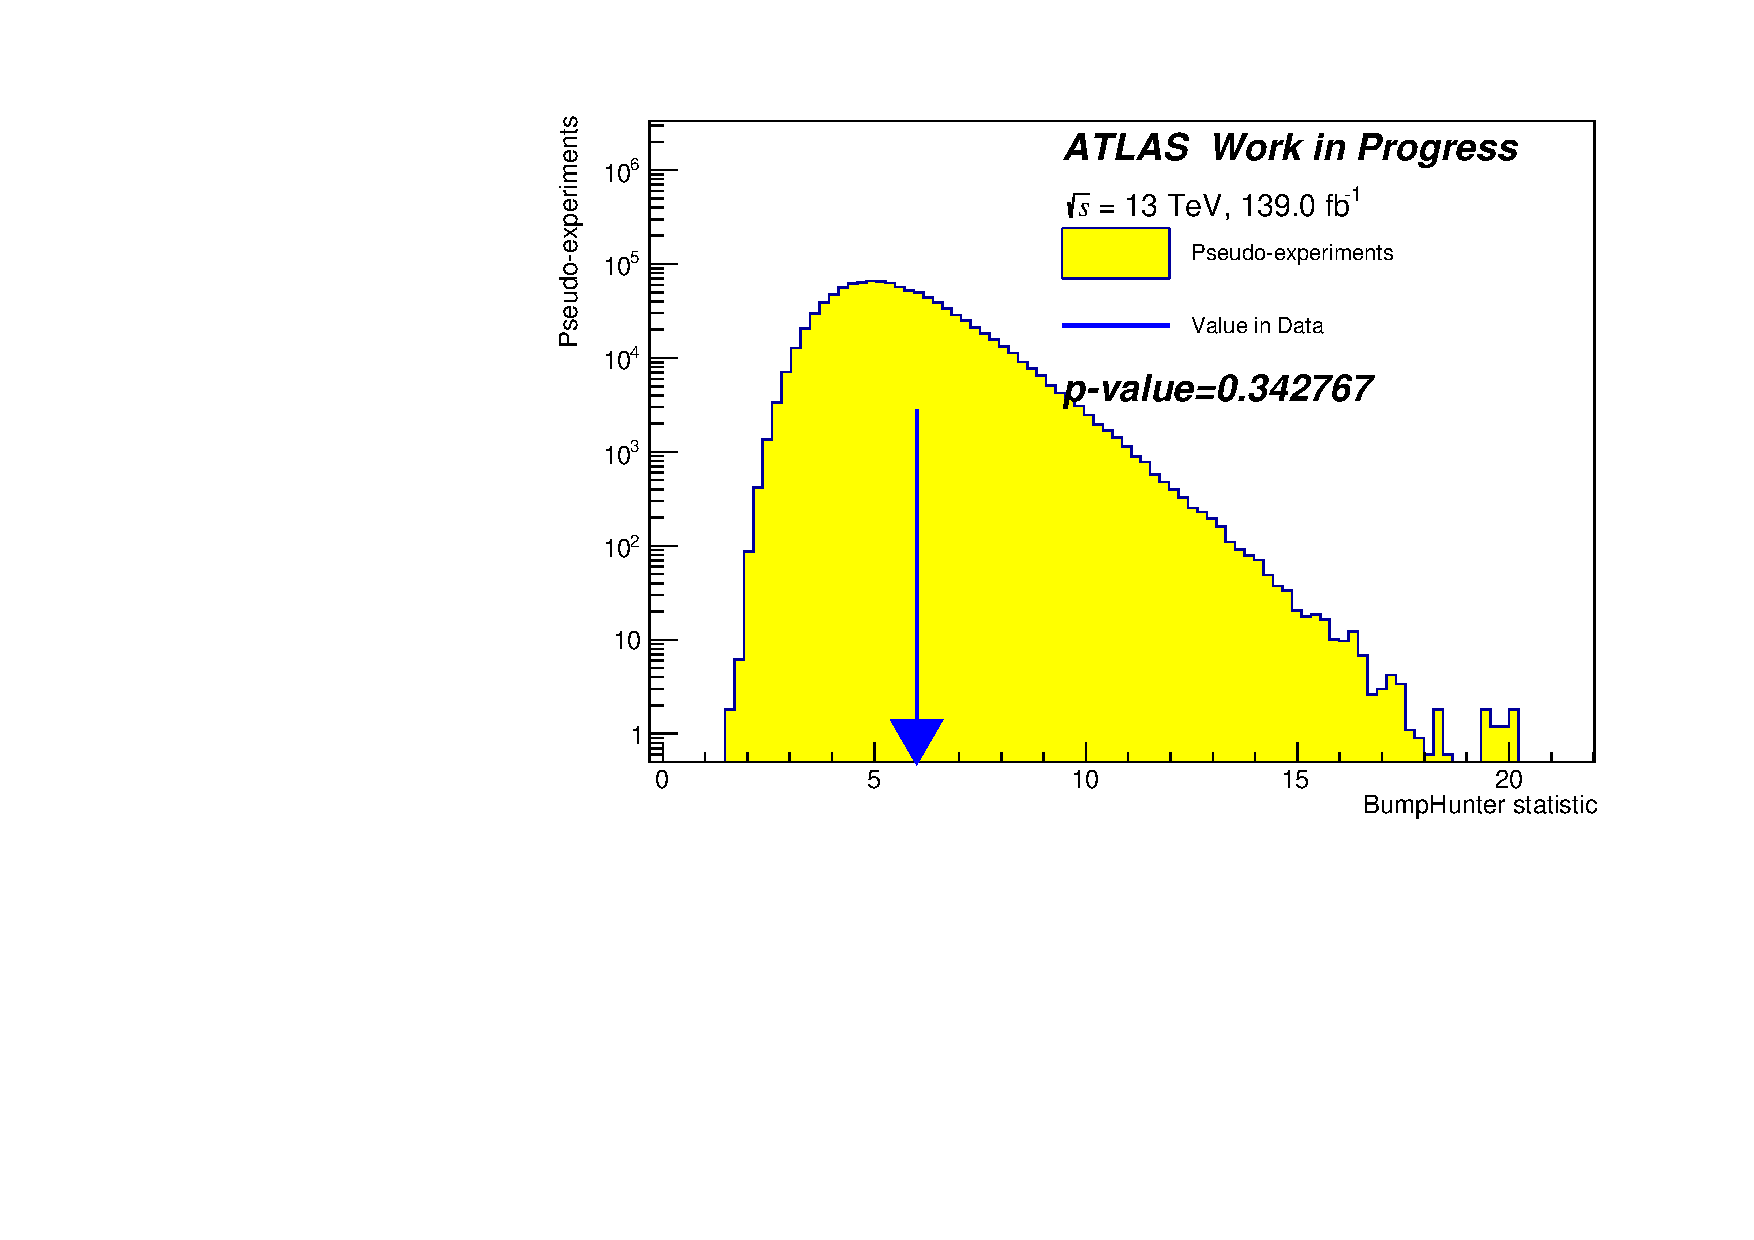
\includegraphics[trim=10 2 35 35, clip,width=1.0\linewidth,height=6cm]{figures/app-GlobalFitStudies/5ParamGlobalYStar0.6_BumpHunterPValue.pdf}
    \caption{Global background fit}
    \label{fig:sub2ystar0.6FullRunBHPvalue}
  \end{subfigure}
  \caption{BumpHunter p-values calculated using BumpHunter for H' cuts inclusive $|y*|<0.6$ data fitted with a 5 parameter dijet fit function fitted both with SWiFt and globally, showing a large difference between the p-value obtained with SWiFt than with global fitting.}
  \label{fig:ystar0.6FullRunBHPvalue}
\end{figure}

\begin{figure}
  \hspace{-3.3cm}
  \begin{subfigure}{.8\linewidth}
    \centering
    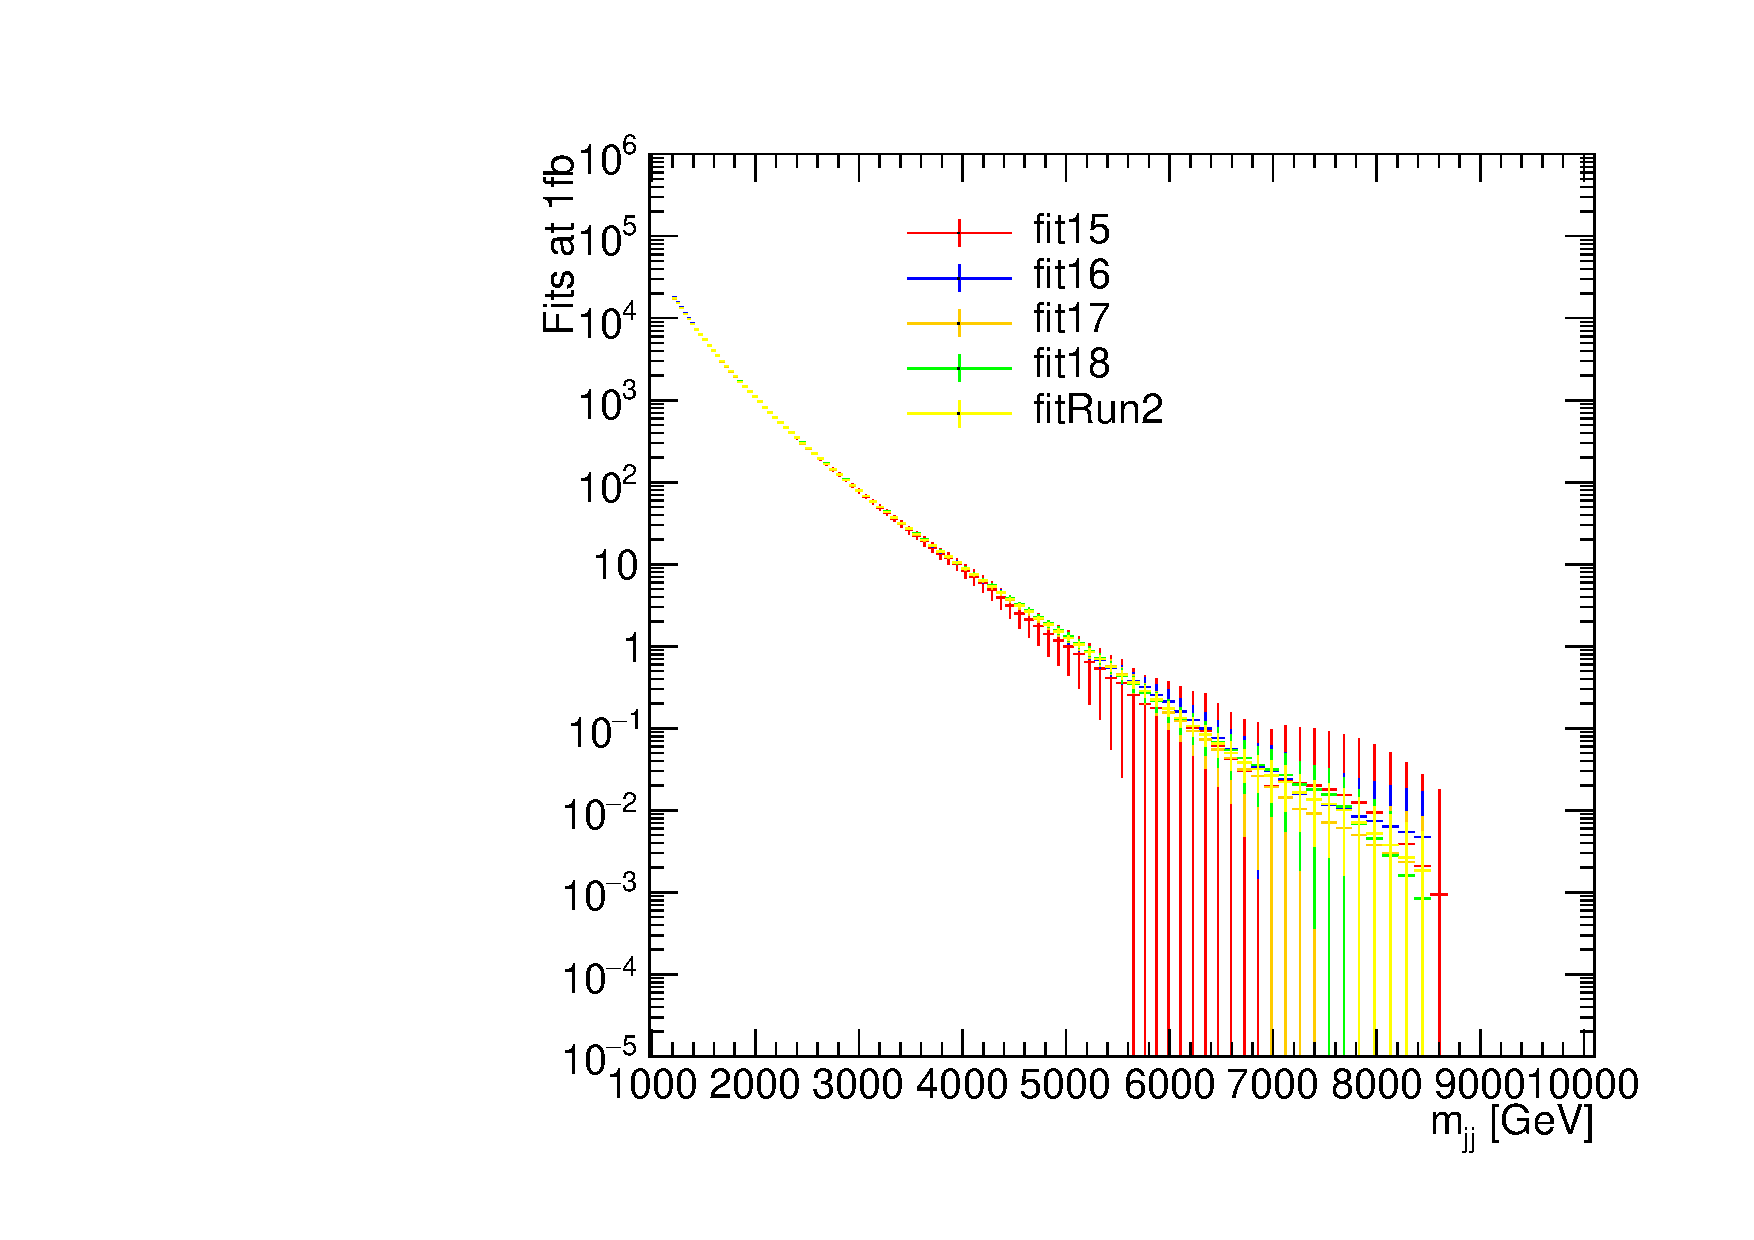
\includegraphics[trim=5 8 14 30, clip,width=1.0\linewidth,height=8cm]{figures/app-GlobalFitStudies/VariousYearsFitsAt1Fb_SWiFtYstar0.6.pdf}
    \caption{SWiFt background fit}
    \label{fig:sub1ystar0.6IndividualFits}
  \end{subfigure}%
  \begin{subfigure}{.8\linewidth}
    \centering
    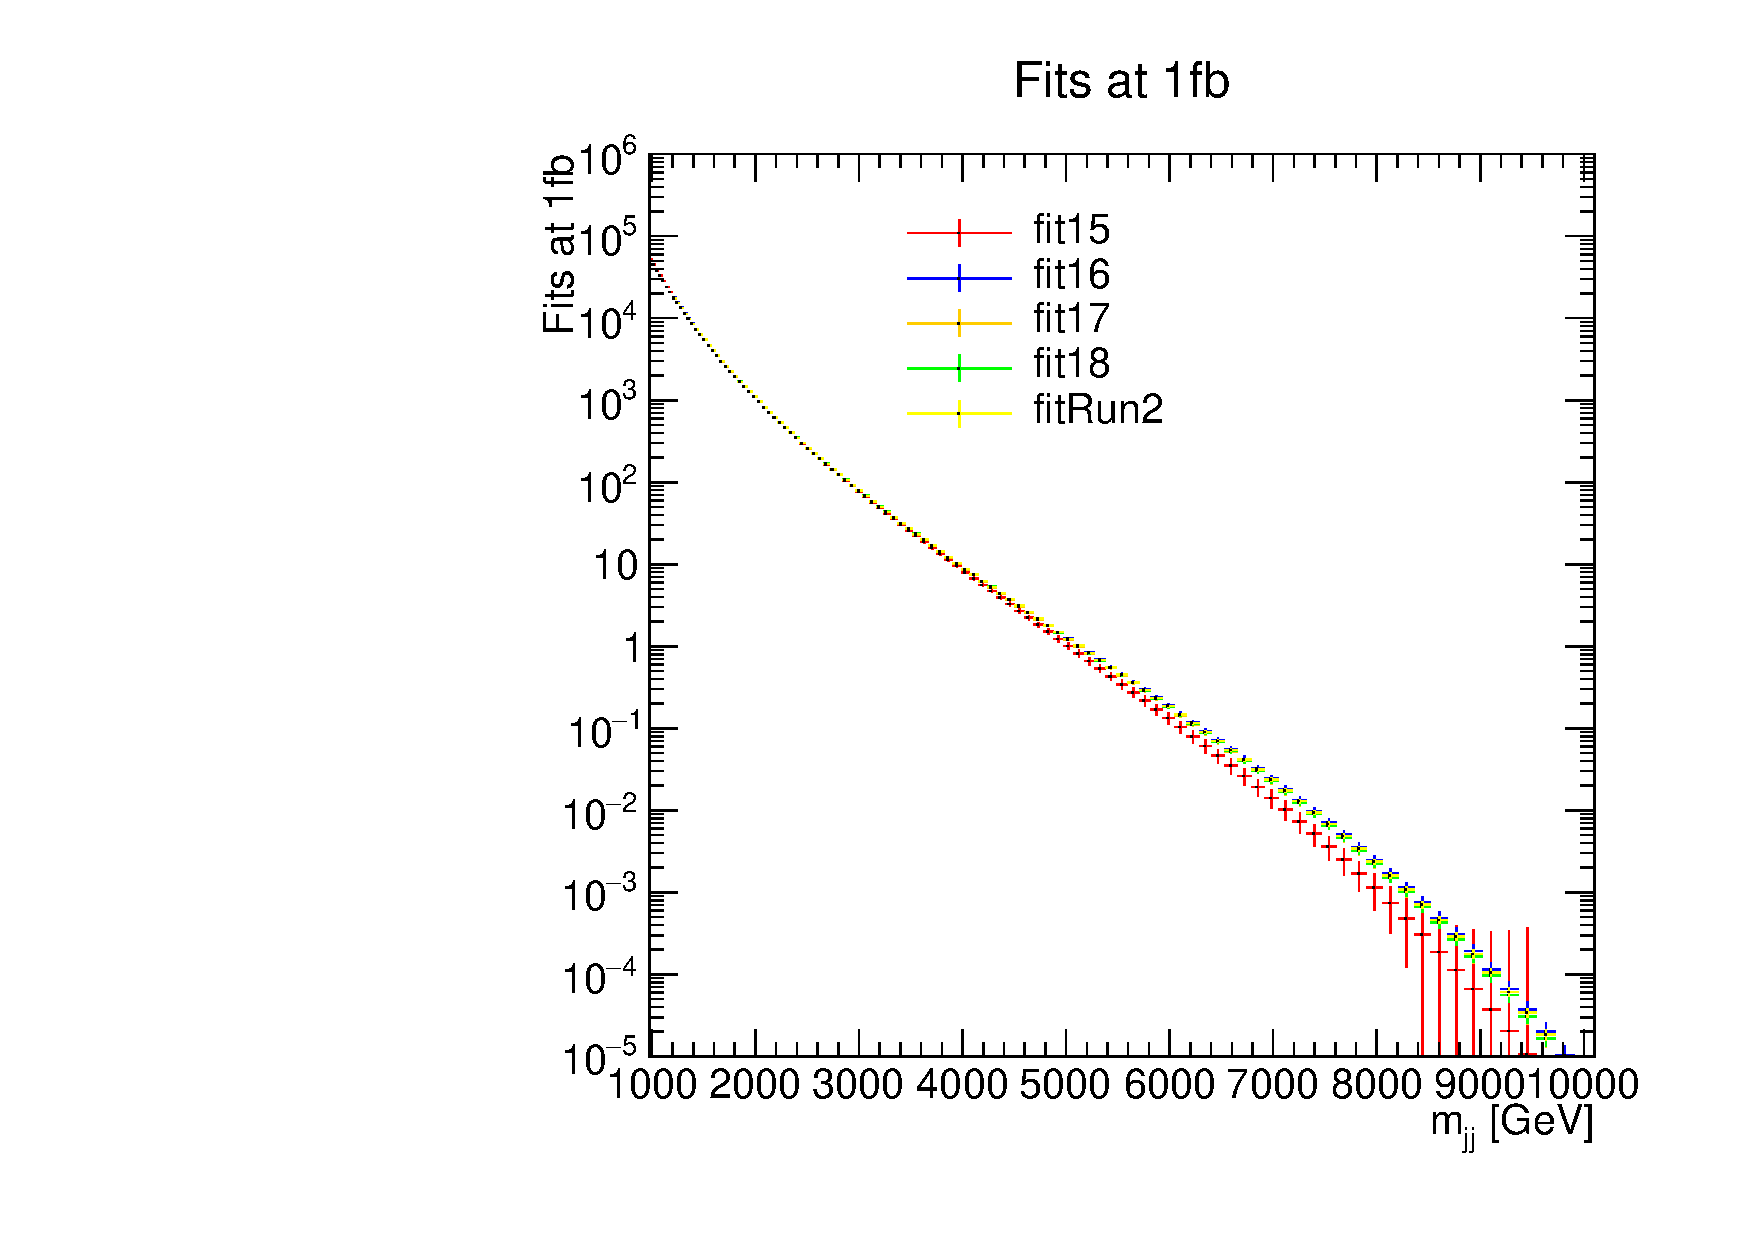
\includegraphics[trim=5 8 14 30, clip,width=1.0\linewidth,height=8cm]{figures/app-GlobalFitStudies/VariousYearsFitsAt1FbYstar0.6.pdf}
    \caption{Global background fit}
    \label{fig:sub2ystar0.6IndividualFits}
  \end{subfigure}
  \caption{Background fit for each year of running in both SWiFt and global fitting, normalized to 1 fb$^{-1}$.}
  \label{fig:ystar0.6IndividualFits}
\end{figure}
